%\documentclass[10pt,a4paper,UTF8]{ctexart}
%\usepackage{graphicx}
%\usepackage{makecell}
%\usepackage{bm}
%\usepackage{amsmath} 
%\usepackage{amssymb}
%\usepackage{amsfonts}
%\usepackage{caption}
%\usepackage{subfigure}
%%导言区域要添加以上两个包
%\usepackage[breaklinks,colorlinks,linkcolor=black,citecolor=black,urlcolor=black]{hyperref}
% \documentclass[cn,chinesefont=nofont]{elegantbook}
% \usepackage{ctex}


% \setmainfont{XITS}  % 英文字体, Times 风格

% \setCJKmainfont{Source Han Serif SC}[         % 方正书宋_GBK
%     BoldFont=Source Han Serif SC Bold,  % 思源宋体粗体
%     ItalicFont=FZKai-Z03                % 方正楷体_GBK
%     ]
% \setCJKsansfont{Source Han Sans SC}[             % 方正黑体_GBK
%     BoldFont=Source Han Sans SC Bold    % 思源黑体粗体
%     ]
% \setCJKmonofont{FZFangSong-Z02}         % 方正仿宋_GBK

% \setCJKfamilyfont{zhsong}{FZShuSong-Z01}
% \setCJKfamilyfont{zhxbs}{Source Han Serif SC Bold}
% \setCJKfamilyfont{zhdbs}{Source Han Serif SC Heavy}
% \setCJKfamilyfont{zhhei}{FZHei-B01}
% \setCJKfamilyfont{zhdh}{Source Han Sans SC Bold}
% \setCJKfamilyfont{zhfs}{FZFangSong-Z02}
% \setCJKfamilyfont{zhkai}{FZKai-Z03}

% \newcommand{\songti}{\CJKfamily{zhsong}}
% \newcommand{\xbsong}{\CJKfamily{zhxbs}}
% \newcommand{\dbsong}{\CJKfamily{zhdbs}}
% \newcommand{\heiti}{\CJKfamily{zhhei}}
% \newcommand{\dahei}{\CJKfamily{zhdh}}
% \newcommand{\fangsong}{\CJKfamily{zhfs}}
% \newcommand{\kaishu}{\CJKfamily{zhkai}}

% \setCJKmainfont[BoldFont={FZHei-B01},ItalicFont={FZKai-Z03}]{FZShuSong-Z01}
% \setCJKsansfont[BoldFont={FZHei-B01},ItalicFont={FZHei-B01}]{FZHei-B01}
% \setCJKmonofont[BoldFont={FZHei-B01},ItalicFont={FZHei-B01}]{FZFangSong-Z02}
% \setCJKfamilyfont{zhsong}{FZShuSong-Z01}
% \setCJKfamilyfont{zhhei}{FZHei-B01}
% \setCJKfamilyfont{zhkai}{FZKai-Z03}
% \setCJKfamilyfont{zhfs}{FZFangSong-Z02}
% \newcommand*{\songti}{\CJKfamily{zhsong}}
% \newcommand*{\heiti}{\CJKfamily{zhhei}}
% \newcommand*{\kaishu}{\CJKfamily{zhkai}}
% \newcommand*{\fangsong}{\CJKfamily{zhfs}}

% \cover{pic/cover.jpg}

\documentclass[openany,twoside,scheme=chinese,fontset=none]{ctexbook}
\usepackage{geometry}
\geometry{
    paperheight=260mm,
    paperwidth=185mm,
    top=25mm,
    bottom=15mm,
    left=25mm, % 左侧留 5mm 装订线距离
    right=15mm
}

\setmainfont{XITS}  % 英文字体, Times 风格

\setCJKmainfont{Source Han Serif SC}[         % 方正书宋_GBK
    BoldFont=Source Han Serif SC Bold,  % 思源宋体粗体
    ItalicFont=FZKai-Z03                % 方正楷体_GBK
    ]
\setCJKsansfont{Source Han Sans SC}[             % 方正黑体_GBK
    BoldFont=Source Han Sans SC Bold    % 思源黑体粗体
    ]
\setCJKmonofont{FZFangSong-Z02}         % 方正仿宋_GBK

\setCJKfamilyfont{zhsong}{FZShuSong-Z01}
\setCJKfamilyfont{zhxbs}{Source Han Serif SC Bold}
\setCJKfamilyfont{zhdbs}{Source Han Serif SC Heavy}
\setCJKfamilyfont{zhhei}{FZHei-B01}
\setCJKfamilyfont{zhdh}{Source Han Sans SC Bold}
\setCJKfamilyfont{zhfs}{FZFangSong-Z02}
\setCJKfamilyfont{zhkai}{FZKai-Z03}

\newcommand{\songti}{\CJKfamily{zhsong}}
\newcommand{\xbsong}{\CJKfamily{zhxbs}}
\newcommand{\dbsong}{\CJKfamily{zhdbs}}
\newcommand{\heiti}{\CJKfamily{zhhei}}
\newcommand{\dahei}{\CJKfamily{zhdh}}
\newcommand{\fangsong}{\CJKfamily{zhfs}}
\newcommand{\kaishu}{\CJKfamily{zhkai}}


\usepackage{amsmath}
\usepackage{amsthm}
\usepackage{amssymb}
\usepackage{hyperref} % \url
\usepackage{graphicx} % \includegraphics
\newtheorem{example}{例}

\title{重修微积分}
\author{应行仁}

\begin{document}
	\maketitle
	
	\newpage
	\tableofcontents
	
	\newpage
	\thispagestyle{empty}
	
	\listoffigures
	
	%\listoftables
	
	\newpage
	
	\pagenumbering{arabic}
	
	\chapter{重修微积分1——无穷}
这个科普系列是给学过微积分及更深入分析课程的人,觉得读书做题考试都还行,但直观和定义隔了一条河,提到严谨只觉得烦,希望能理解现代分析,又能像物理那样想象的同学。这里介绍无穷、拓扑、空间、测度、泛函和算子等现代分析的概念,让你从高处来看风景。

我学过几次微积分。最初是在高中,了解了导数是变化率,积分能算面积,它们互为逆运算。接着翻到微积分书里的求导公式,一口气背下初等函数导数表和复合函数公式。凭着这个直观概念和套公式本领,大学物理公式推导也看懂了,几天时间里武功大进,高中各种难题,触手可解。这时心雄万夫,认为这就是微积分了。想不明白那巨厚的教材,花那么多的篇幅整什么极限和收敛?后来了解到很多人也和我一样,就学个招式套路,没得心法真传,思想还是停留在有限数学的圈子里,没有走过用逻辑搭起越过无穷深渊的桥,所以永远无法想象不能感知的世界,所说的也只是人云亦云,对与错,自己是无法确认的。再学的实变泛函随机过程,即使考分不错,也只是学个技巧能够解题。真正去应用则在云中雾里,心中懵懂始终不觉踏实。直到在美国数学系从点集拓扑重新学起,每一步踏实了走过去,在巨细的习题中摸过每一块石头,才重新建立起直观想象,找回了自信。

工程师和非数学研究者,不可能都沿着纯数学的路子学习现代严谨的数学理论。耗费大量时间在逻辑巷道里穿行,会让你失去方向看不到全貌,不一定所有人都能走通。对大多数人,数学只是个严谨的逻辑建筑模块和工具。想用好它,最重要的不是繁琐的条件和证明细节的了解,而是要有正确概念的理解。有了正确想象,即使不能精通现代分析,你也能大致读懂相关的理论,用定理套公式才能有自信。急用先学恶补知识时也会有方向。

从初等数学到数学分析,是从现实世界到了无穷空间的跃迁。在牛顿之后,学术界也曾经为此想象图像的转变,迷惑混乱了几百年,至今书里和教授传承还遗留着许多当年混战中的繁杂解读。要走过这座桥,你必须超越有限世界经验的局限,用逻辑证明过的典型例子,来构筑无穷世界的直观想象,知道为什么要分辨看似无谓的概念,接受经验不习惯的事例,才能到达彼岸。

这系列短文,不是教程,而在解读概念。如果你学过这些课程,这里让你依想象指引用逻辑将概念和例子串起来,没学过的也可以浏览无穷世界里的风光。希望有助于迷惘中的人,纠正错误的观念,建立较正确的直观想象,明白些为什么,想穷究深入时,知道往哪儿找。



在微积分之前,数学几乎都是关于“有限”的学问,因为只有是有限的个体,或是它们的有限组合,才算得了,说得清。归纳是人类智力的本能。使用数学归纳法,能够把只对有限事例成立的结论,依仗逻辑和递推关系,严谨地推广到无穷多的适用情况。许多人以为这已是无穷的世界了,其实这只是这个词的一种意思,仍然是在有限的世界里兜圈子。无穷在这里指的是:这个递推过程可以是无法穷尽的。这个认知叫“潜无穷”。在这个无穷尽的过程中,你接触到的每一个还是有限的个体,推理的正确性也只是针对这过程中经过的每一站,无穷的过程没有终点,它们的全体不在考虑之列。

\kaishu
\setlength{\leftskip}{1em}
例如:集合$ \{1\} $是有限集,假如 $ {1,2,\cdots,n} $ 是有限集,那么多一个元素的 $ \{1,2,\cdots,n,n+1\} $ 也是有限集,根据数学归纳法,这对所有n都成立。但这不证明所有自然数的集合$ \{1,2,3 \cdots\} $是个有限集。因为数学归纳法的证明,对所有自然数都成立的命题,是一种潜无穷的陈述,是动态地指对每一个具体的自然数能成立的陈述,而不是指对自然数的全体都成立。

\songti
\setlength{\leftskip}{0em}
有限的度量是实践中可以验证的,潜无穷是以此推理的极限。在物理世界,能够被检验和推测的数量,都是有限精度或组合的;任何计算,都必须在有限的步骤中终止,才有结果;数学证明,必须在有限步骤的推理中完成,才是可信。一句话,现实的世界本来是有限的。人们固有的直观想象,都是在有穷的世界里,用实践经验累积和事例验证而成的。

我们现在普遍认知的连续无限可分世界,是微积分这个数学工具成功应用后,人们在书本灌输下接受的假设。这个看似已经深入人心的观念,对绝大多数人只是个不断被重复的表面陈述,与学前的直观不能融合,难以深思。无穷的彼岸和有限的经验是完全不同的两个世界,归纳法的逻辑无法越过有穷的边界。我们必须先验地承认某些无法验证的观念,用逻辑构造出包囊一切的统一图像,才能消融这个隔阂。

无限的过程能否成为一个数学的量?这早在两千多年前的古希腊,就引起争论,它实际是哲学上的一个观念。无法验证也无关对错。数学是个关心在给定前提下,依照逻辑推理能够走多远的学问。古希腊的毕达哥斯学派,还有个追求的指标是“美”,和谐的美、统一的美、简洁的美。主张无穷不仅仅是个变动的过程,而且这无限过程,代表着它要达到的数学实体,可以用来参与计算,称之为“实无穷”,是把它作为一种数学完备化的扩张。

认为无穷不仅仅是一个过程,而且代表着一个要达到的数值,这在逻辑上很重要。只有这样我们才可以把它放在等式里。比如说,认为无穷循环的 $ 0.999... $ 是数x,才有$ 10x=9.999\cdots $,因此$ 10x = 9 + x $,得出$ x = 1 $. 阿基米德用了同样的原理,将阿基里斯追逐乌龟的过程,写成无穷级数的和$ 1+0.1+0.01+0.001+\cdots $,把它当作一个数x,由$ 10x=10+x $关系,才能算出他追上乌龟在x=10/9处。牛顿和莱布尼茨定义导数为两个无穷小量dy和dx之比dy/dx,到了后来柯西修正为导数是Δy/Δx分子分母都趋于0的无穷过程。这些都只有承认实无穷观点时,才有可能。

这些都是假定实无穷能够保持算术运算的和谐关系,才得出答案的。历史上数学天才运用这个思想,取得了令人惊异的成绩。但是这个扩张并不总是像引入开平方的无理数那样和谐。1703年,意大利数学家格蓝迪问大家,无限的过程$ 1-1+1-1+1-1+\cdots $,等于多少?数学王子欧拉,用阿基米德相同的方法,假设$ x=1-1+1-1+1-1+\cdots $,将这个无限过程第一项1先拎出来,后面剩下的相当于它自己乘上-1,有了$  x=1-x $,欧拉得出格蓝迪级数的和是1/2。但是有人说,根据加法的结合律,有$ x=(1-1)+(1-1)+(1-1)+\cdots=0+0+0+\cdots=0 $,类似的做法还可以有$ x=1+(-1+1)+(-1+1)+(-1+1)+\cdots=1+0+0+0+\cdots=1 $。这格蓝迪级数到底是0、1/2还是1?贝克莱主教质问牛顿:你这个无穷小在做除法时认为不是0,在做加减法时当着是0,它到底是0还是个非0的数?

其实古人早已疑惑:自然数全体的数量是无穷大,在其中拿掉几个数,它还是一样大吗?无穷循环小数 $ 0.999... $的每一个截断都小于1,它怎么最终不再小于1?承认和不承认实无穷的存在,都与某一种数学的美相冲突。这就是数学家在历史上,对实无穷和潜无穷无所适从的原因。

在牛顿之前,数学家对实无穷采取回避的态度,除了个别公认的天才,有底气做别人不敢质疑的猜测,大家都只老老实实地把无穷只看是一个过程,这样心里踏实,这也是潜无穷派的想法。但微积分是关于无穷的算术。到这时已是无可回避了。

这些冲突,实际上是企图将本质不同东西纳入过去直观的框架。对于有穷的东西,我们可以验证它,从已知的数学实体中通过有限步的推理确认它。在实无穷与确定的数之间,却没有能够确信的桥梁。无穷的序列,可能等价于已知的数学元素,也可以不是大家熟悉的东西,也可能是非此非彼的不确定。把本质上不能一致定义的东西,放入有限数学通行的等式里,从不同的方向则会推出不同的东西。这便是发生矛盾的原因。

现代数学基本认可实无穷的观念,但不认为它的所指都有意义。这个无限的过程,并非都能代表一个数。有的不是指向大家熟悉的数学元素;有的并没有确定的数学意义。实无穷的提法,因为涉及过多历史上混乱的争议,在数学界也不再强调了,而着眼于具体的处理。

将实践中无法检验的一种概念作为构筑理论的砖块,在思想史上并不罕见。在哲学、宗教、社会科学、甚至在自然科学理论里比比皆是。人们希望用新概念的理论,能够透视现实中的秘密,用之推演的结果,与我们的观察有某种程度的吻合。数学家的任务是将它精确化,限定适用的范围,以保证在逻辑上不至于造成冲突。科学是用逻辑为混沌的自然立法,让世界看起来比较有条理。

集合论作为现代数学的基石,研究了无穷大这个新的数学实体。它用一一映射的关系,回答了无穷大比较的问题。这个无穷大与有限的数,只保持一种序的关系,它们是不在一个层次数量,有限数的运算不完全适用于它。这提醒人们,不能用处理有限世界的那种直观,来看待用逻辑扩张出来的无穷世界。要自信自如地在这世界里玩,你必须理解新的概念,接受一些不习惯的事例,用逻辑推演出来的事例来纠正旧的想象,形成新的直观图像。

用无穷变化的过程代表一个可以达到的数,这需要另一座桥梁,我们必须知道这是在什么意义下的等价关系,在什么条件下才有可能,这需要理解一个概念——收敛。
 	\chapter{重修微积分2——收敛}
无穷序列可以用来表示一种趋向。其思想仍然与归纳法一样,企图用已知来推测未知。这里是用有穷的序列项来推测无穷之处的结果。只不过数学归纳法,只能在有穷的世界里漫行,这里需要一个假设,才能用逻辑跨过边界。

大致地说,无穷序列作为数学的模型,在这无穷过程中,当后来的项越来越相像,如果这无穷过程指向一个实无穷的极限,设定的含义是:这极限与有穷过程里的项,也将会是越来越相像,以致难以区分。在这种情况下,我们有把握确定这个极限的性质,可以用这个无穷过程来定义或确定这个极限。

这里有两个问题。一是这序列能否指向一个数学实体,二是什么叫做``相像''。

第一个问题,不外乎三种情况。一是不能。那就飘过。但如果是都不可能,那就不用谈极限了,微积分是个梦,大家仍旧玩算术。二是指向未知的实体。我们也许可以用模型里``相像''这性质来定义它,叫做扩充。这押后再谈。三是指向这空间里已有的实体,称之为收敛的极限。因为它与序列中的项同在一个空间,它们在空间里的关系可以用来描述``相像''的含义。

以上所说并不限于实数,适合于包括函数、事件,以及集合元素的无穷序列。不同的``相像''含义,确定了不同收敛和极限的含义,这将在以后的篇章里展开。请记住这里的图像,作为分析中直观想象的基础。这一篇,我们先谈最简单的情况——数列。

对于数而言,现实的计算只能区分有限精度的数。按照某种精度画个圈,一个无穷的数列,除了前面有限多个外,如果此后所有的项终将全部落入这个圈里,按照这数学模型的假设,它指向的极限,也是在这圈子里。在这圈里任何两个数,按这精度看不出区别,在圈里取任意一个数当作那个极限也是如此。如果总能以任何精度做到这一点,也就能以任何精度确定这个终极的数。这个无穷数列就对应着这个数。

如果这个极限在讨论的空间上存在,这数列称为``收敛''到这个极限。

用数学语言表达无穷数列$ (x_n) $收敛于a是: $ \lim_{n\rightarrow \infty} a_n = a $ 或者写成 $ a_n \rightarrow a , \mbox{ } (n \rightarrow \infty) $ ,在不混淆的情况可以略去括号里n的走向。上述收敛的定义用 $ \varepsilon -N $ 语言和数理逻辑符号表达是:
\begin{equation}
	\forall \varepsilon > 0, \exists N \in \mathbb{N},\forall n ( n>N \Rightarrow |a_n-a| < \varepsilon )
\end{equation}

这定义只是说,如果有个数符合这描述,则称数列收敛于它。要认为这个无穷数列确定了这个数,需要证明它是唯一的。作为数学模型的要求,我们还必须证明,收敛的极限与空间里的数做四则运算,其结果与用数列中的项参与同样运算的数列极限是一样的。这些证明都不难,最后都归结为:要验证的差异随着N足够大也会小于任何正数。即这个差异的无穷数列无限地趋向0。所以在极限时等于0. 停!在这句结论之前,全部是对有穷数列的推算,这无穷数列要走过所有的项,才能得出相等的结论,这需要一个假设,才能越过这个逻辑的间隙:无穷必须是可以完成的!这样无限减小又始终存在的差异才会消失,让无穷序列的桥梁能够搭上有限世界的对岸。这是被许多人忽略,以致缺乏动力去改变有穷世界里的直观。

从收敛的定义不难看出,如果无穷过程收敛,那么在这过程中走得足够远的项之间的差别也会足够小,即
\begin{equation}
	\forall \varepsilon > 0, \exists N \in \mathbb{N},\forall n \forall m ( m,n>N \Rightarrow |a_n-a_m| < \varepsilon )
\end{equation}

这样的数列 $ (x_n) $ ,叫做``柯西列(Cauchy sequence)''。能够收敛的数列都是柯西列。

回头来看格蓝迪级数1-1+1-1+1-1+…,这个无穷过程无法确定任何数值,其有限和构成的无穷数列不是柯西列,不能收敛。欧拉和在收敛意义上不成立。

并非所有柯西列都能收敛,它取决于所在空间的性质。例如,$ \sqrt{2} $

取越来越多位数的数列1.4,1.41,1.414,… 是柯西列,但它在有理数空间不收敛。即这个数列极限在有理数中不存在。

能够让所有柯西列都收敛的数学空间,叫做``完备的(Complete)''。微积分发明之后,数学家又发现了大量未知的实数和并严格修补了实数的定义,从而证明了实数是完备的。这表示只要数列是趋于相互靠拢的,就一定有极限,这个意义很重大。初等微积分是建立在实数完备性的基础上。

实数在近代,是用有理数上戴迪金分割来定义,把有理数集分割成上下两个集合,让上集合中所有的有理数,都大于下集合的;无理数被定义为,填充这种分割中的``间隙''。可以证明,这样定义的无理数和有理数,构成的实数,在收敛的意义下是完备的。

实数在传统上,看成整数加上一个无穷的小数。一个无穷小数,取越来越多位数的过程,是个柯西列,如果定义这个无穷过程表示的数学实体叫做``实数'',这时,实数可以看成是有理数的完备化扩张。

不论是怎样构造的,它们是等价的,实数是完备的,所有的柯西数列在实数上都收敛。

下面是几个微积分上熟知的定理,说的都是实数的性质,可以证明它们是互相等价的:

\kaishu
\setlength{\leftskip}{1em}
\begin{enumerate}
	\item 实数是完备的。
	
	\item 实数任意上(下)有界的集合,一定有上(下)确界。
	
	\item 单调有界的数列有极限。
	
	\item (区间套定理)闭区间序列$ ([a_n, b_n]) $	,如果$ [a_n, b_n]\supset [a_{n+1}, b_{n+1}], \forall n \ge 1  $并且 $ (b_n-a_n)\rightarrow 0 $ ,则必定存在着唯一的实数c有 $ c \in [a_n, b_n],\forall n \ge 1 $ ,并且 $ a_n \rightarrow c $ 和 $ b_n \rightarrow c $ 。这个闭区间序列叫作``区间套''。
	
	\item (有限覆盖定理)有界闭区间I上的任何开区间覆盖族中,必定有一组有限的开区间覆盖I。
	
	\item (列紧性定理)任何有界数列必定有一个收敛的子列。
\end{enumerate}

\songti
\setlength{\leftskip}{0em}
采用戴迪金类似的方法,是否还能发现实数间的空隙?从实数的完备性,可以证明了这样的空隙不存在。这也称为实数是``连续的''。

任何两个有理数,无论之差是多小,其间都有不可数个实数。只有夹在一个无穷地不断增大的有理数列,与另一无穷地不断减小的有理数列中,当它们之间的差值趋向0时,其``缝隙''才只够容下一个实数。

实数的完备性是微积分的基石。与此等价的上述性质,在微积分中扮演了重要的角色。

康托尔用对角线法证明了,实数是不可数的。从实数完备性上,也不难证明实数是不可数的。

\kaishu
\setlength{\leftskip}{1em}
用反证法。假设闭区间[0, 3]里的实数可数,那么可将它们标记为:$ x_1, x_2, x_3, \cdots  $。将$ [0, 3 $]等分成三个区间 $ [0, 1], [1, 2], [2, 3], x_1 $必然不在其中之一,记这区间为$ I1 = [a_1, b_1] $,再将$ I_1 $等分成三个区间,同样必有一个子区间不含$ x_2 $,记这区间为$ I_2 = [a_2, b_2] $,如此进行下去,得到一个区间套$ I_1, I_2, I_3, \cdots $。根据区间套定理,存在着一个实数y在所有这些区间中。但从区间的选取中知道,$ x_n $不在$ I_n $中,所以实数y不是$ x_1, x_2, x_3, \cdots $中任何一个。这就和假设相矛盾。所以实数是不可数的。

\songti
\setlength{\leftskip}{0em}
实数必须是不可数的,才不会与它的完备性相冲突。在可数的世界里,没有微积分。

对于古希腊毕达哥斯派的疑问:无穷循环小数0.999…的每一个截断都小于1,它怎么最终会等于1?从对于每一个截断所有n都成立的命题,得出对全体也成立的结论,是有穷世界直观的错觉。持潜无穷的观点,0.999…只是个无穷的过程,这小于的关系永远存在,当然不会等于1。但是这里的``所有'',指的是对每一个有限的数n,而不是包括了它们无穷全体的``最终''。就像上篇的数学归纳法的例子,这个对所有n的推理,只在有穷世界里是对的。不能应用于无穷。这是必需改变的观念。按实无穷的观点,这个无穷的过程是可以达到它的极限,也就是等于1,这小于的关系,因达到极限而终结为相等。收敛的极限可以等于比数列中每一项都大(小)的上(下)确界。

柯西和魏尔斯特拉斯之后的微积分,为了避免过去对实无穷的简单解读,在能够用潜无穷观念解释的地方,尽量避免使用实无穷。但对收敛的极限,逻辑上毕竟不能绕开实无穷的观念。

也许大家觉得上面所说的内容很浅,早在学习微积分时就知道了。好,考个对收敛理解的问题。

\kaishu
\setlength{\leftskip}{1em}

张三找李四寻仇,拿个炸弹设了一分钟后扔向李四,李四半分钟后扔回,张三在四分之一分钟后又扔向李四,如此往复,问最后炸弹在谁的手里爆炸?

(停下思考5分钟,再往下看,再思考。)

如果知道某个时刻落在这个无穷往复过程的哪一个时段,就知道炸弹在谁的手里。虽然这是个无穷的过程,但爆炸的时刻终将会到来。这些时段的累加为1/2+1/4+1/8+……,级数收敛到极限1。但时刻1在这些描述炸弹位置的时段里吗?这个数学模型能描述现实的情况吗?

\songti
\setlength{\leftskip}{0em}

【扩展阅读】

\begin{enumerate}
	\item 实数理论 \url{http://210.26.16.17/ziyuan/38/analysis/precis/Acrobat/21.pdf}

	\item 实数的完备性 \url{http://210.45.128.5/jpkc/shuxiefx/sxfxky/hky.pdf}
\end{enumerate}

 	\chapter{重修微积分3——拓扑}

上一篇探讨了实数收敛的概念,用无穷级数来确定一个数。很容易把它扩展到无穷的函数序列求极限的问题。在初等微积分里,这是对函数变量的每个值逐点来考察,对每个固定的变量值,这无穷序列对应着一个函数值的数列,如果所有点对应的数列都收敛,那就认为这无穷函数序列收敛,它的极限函数在每个点的函数值是相应数列的极限值。这样函数序列的极限称为逐点收敛的。这个方法被牛顿引入后,广泛地应用,它虽然可行,但在微积分进一步研究时又遇到种种麻烦,于是又附加了许多条件,如“一致连续”,“绝对可积”等等,最后弄得微积分繁杂不堪。能不能把整个函数看成一个数学空间里的一个点,把这些条件都看成空间里的性质,从一个统一的角度来研究收敛极限的问题?这便是这一篇要介绍的概念。

现代的数学建立在比实数更加抽象的集合论基础上,应用于更广泛的空间。要将定义在实数上一元函数微积分的本质说清楚,推广到多元函数,函数逼近,泛函,随机过程,乃至各种抽象数学结构的集合上,我们要了解集合元素间联系的结构,这样才可能描述变动个体的走向,空间的性质,进而谈及趋近、收敛和极限。

微积分是基于无穷逼近极限的数学。收敛描述的是变动差别越来越小,直至微不可察的数列表现。收敛极限的存在,取决于实数的完备性。所以无穷逼近过程的含义和结果,依赖于它所在数学空间的性质。传统微积分是建立在实数空间R

的性质上。这些实数性质是人们在习以为常的计算经验中总结“发现”出来,又用一些更简单基本的原理来证明的。

在现代数学之前,数学一直被认为是研究真理的学问,直到百多年前,哲人们还都认为不但如此,而且是绝对的真理。现在看来,这些真理也许不过是:习惯成了自然的经验在逻辑上自洽的表现。几千年实践认知形成有穷数学的直观与那时的理论吻合无间。无穷则无法验证,除了凌空而来的假定和逻辑自洽之外无所凭借,一切概念和引为依据的原理都需要精确的定义引入,一切的争执最终也只能根据这些定义和假设,用逻辑作出判决。直觉、经验、试验和公认之事,对数学都不足为凭。数学的价值在于有用,在虚构的空间里,以严谨的逻辑铸造出一把犀利的思想宝刀,当你用对了,无数的实践难题可以迎刃而解。

要想自如地在在抽象的无穷空间中行走,你需要正确的直观想象。前面两篇只是个导引,让你意识到必须纠正过去的直觉,才能放开心怀接纳无穷空间里的真实。在“无穷”篇里数学归纳法的例子,证明了在有限情况都成立的论断,在无穷时未必成立。要走出有限的误区,才能走出局限。在“收敛”篇里0.999…=1的分析,说明了极限的含义。这是微积分数学模型的最基本假设,无穷过程达到彼岸的立足点。所有收敛的极限都是依相同的原理,将差异的不等式在极限处变成了等式。除非你曾经震惊思考改变过,如果初读前面这两个例子,没有经历过困惑,思考到终于理解了,你大约还没有走出有穷世界的藩篱。建议你回去走通了再来,否则学过的微积分知识只是别人说的,不是自己会的,此后三篇让你构筑无穷空间想象的介绍,就可能格格难下不能吸收,无缘看见彼岸。

直觉是模糊的联想,并非精确可靠。别人说的风景和你所想的也许不是同一个地方。只有踏在共同之处才是真实的一样。想象必须依附于证实过的判断作为立足点,只有在坚实的桩脚附近延伸,才靠近真实,过度延伸的浮想只是梦呓。可靠的直觉来自大量被证实过的事例,它们编织成了图像,越多的事例,才有越清晰的直觉。在现实有穷的世界,这些事例来自日积月累的学习和实践,判决正误唯有实验。在抽象无穷的空间,可靠的事例来自符合定义的例子和严格证明过的判断,在这里逻辑是唯一的判据。你必须记忆概念的定义,消化例子,纠正限于有穷世界的直觉,才会形成在无穷空间里的正确直观。

这一篇黑体字强调的概念,如开集、闭集、邻域、收敛、稠集、连续等等,你可能已经认识,不过在初等微积分学的是在实数上的定义,这儿是从抽象集合的高处俯视。这篇把点集拓扑的基本概念串起来介绍,有足够的信息让你可以依想象,走通从定义到例子的逻辑。希望你从过去的认知起步,以这里的定义来消除局限,用例子来校正偏差,在走通的过程中重建图像。花费时间逐个概念走过,你将会开始有看清无穷空间景象的基础。

好吧,抽象!讨论问题的空间一切属性都需要定义。忘掉实数、无穷、收敛、极限种种课堂灌给我们前人发现的真理,从简单干净的抽象集合开始。上一篇说,无穷序列作为数学模型来描述收敛的观念,序列中的项以及极限之间的“相像”性质,决定了收敛和极限的含义。好的。对集合中的两个元素,比如说是两个人,你能从其一了解另一吗?不能。因为元素只是集合中抽象的个体,没有它们间关系的信息。如果说知道它们同在某一个子集里,好比说知道两人同是一族,你就能知道,他们比不在这子集里的外族人有某些更相像。在这里用子集表达其中的元素具有某些共同的属性,这样的子集称之为开集,它们的并和交满足某些封闭性。集合上有了这样的一组开集,便能以此判断元素间属性是否相近。可以用来判别相邻性的这组开集,称为集合上的拓扑,它们组成了讨论无穷逼近问题的数学空间。

\kaishu
\setlength{\leftskip}{1em}
考虑集合X上的一个子集族$ \tau $,其元素是X的子集,如果它们任意多的并,及有限个的交都属于$ \tau $,空集和X也属于$ \tau $,那么 $ \tau $ 中元素称为\textbf{开集}, $ \tau $ 称为X上的\textbf{拓扑(Topology)},组合$ (X, \tau)$称为\textbf{拓扑空间},在简略$\tau$不致混淆时,也可直接称X为拓扑空间。

\songti
\setlength{\leftskip}{0em}

在任何拓扑,空集和X都是开集,只具有这两个开集的拓扑,称为\textbf{平凡拓扑}。取X上的一组子集,包括空集和X本身,定义它们为开集,进而将它们任意多的并,及有限的交,都视为这空间的开集,则生成了一个拓扑$\tau$。给几个实例来帮助想象。

\kaishu
\setlength{\leftskip}{1em}

\noindent
例3.1:定义实数上的开区间为开集,在它们间进行任意多的并和有限个交运算,依定义这生成了实数上的拓扑。通常实数空间指的就是以此为拓扑的空间。

\noindent
例3.2:在闭区间$ [a,b] $上所有连续函数的集合$ C[a,b] $,对任意的 $ f\in C[a,b],\;\;\delta \textgreater 0 $ 
,定义集合 $ \{ g \in C[a,b]\; |\; \max_{a\leq t \leq b} |g(t)-f(t)|<\delta\} $ 为开集,它们任意多的并和有限个交,生成了$ C[a,b] $空间上的一个拓扑。

\noindent
例3.3:集合$ X=\{a,b\} $,定义空集$\phi$,单点集$ \{a\} $和X为开集,它们构成X上的一个拓扑。

\noindent
例3.4:将X上所有子集都定义为开集的拓扑,称为\textbf{离散拓扑}。它也可以由定义任何单点集都为开集来生成的。

\songti
\setlength{\leftskip}{0em}

拓扑空间$ (X,\tau) $中集合X称为空间,它的子集简称为集合,X的元素称为点,点之间的相邻关系,由$\tau$来确定。两个点,如果同在拓扑空间的一个开集里,认为它们是相邻,分属两个不相交的开集,认为是分离;包含了点x的开集,称为x的\textbf{开邻域},包住x开邻域的集合称为x的\textbf{邻域}(neighborhood),寓意是与这点某些属性相近的点都在这里。

那么,怎么用拓扑来描述趋近状态呢?

对于拓扑空间X的一个点x和序列$ (x_n) $,如果对于x的每个邻域U,都有对应着它的一个正数N,当$ n \ge N  $ 时,都有$ x_n \in  U $,则称$ (x_n) $\textbf{收敛}于x。考虑到点的邻域含义,这意味着,对这空间中拓扑所考虑的属性上,这序列后面的点终将与点x是密不可分的。

对于拓扑空间X中一个点x和集合A,如果x的每个邻域都包含有除了x外,还有A中其他的点,则x称为A的一个\textbf{聚点}(cluster point)。例如:在实数空间中,0和1是开区间 $ (0, 1) $的聚点;任何一个无理数都是有理数集的聚点。

显然,序列收敛到非序列中的点x,是序列所在集合的聚点;但集合A的聚点,未必有集合中的序列收敛于它。如果集合中的点都有一组可数的邻域,这点所有邻域都包含这组的某些成员,这样的拓扑空间称为\textbf{第一可数的}(first countable)。第一可数空间集合中的聚点都有集合中的序列收敛于它。在分析应用中的聚点都是用序列来逼近的,所以应用中的拓扑空间都是第一可数的,它也称为可数性的第一公理。

开集的补集称为\textbf{闭集};包住集合A的所有闭集的交,是包住A的最小闭集,叫做A的\textbf{闭包}。闭包也是包括了A和它所有聚点的集合。实数是有理数的闭包。闭区间[a.b]是开区间(a,b)的闭包,闭区间[1, 3]是集合 $[1, 2)\cup $  $(2, 3) $的闭包。

对拓扑空间X的子集A,如果任何开集都包含有A中的点,则称A是X中的\textbf{稠集},意味着X中的点的任何邻域,都含有A中的点,即可以用A中的点来逼近。如果X有个稠集是可数的,则称这空间是\textbf{可分的},X中的点都有这稠集中的一个序列收敛于它。有理数是可数的,它是实数上的稠集,所以实数空间是可分的,每个实数都有一个有理数的数列收敛于它。所有实数都是有理数集合的聚点,实数空间的拓扑是第一可数的。

同一个集合X上可以定义不同的拓扑。平凡拓扑是最粗的拓扑,离散拓扑是最细的。开集设定了一个点的邻域,它意味着里面其它点与这点相类。邻域之外就有某些的“不相类”,所以空间的拓扑区分的能力也很重要。如果对两个点,总有一个点开邻域不含另一,称为$ T_0 $空间;它们各自都有不包含对方的开邻域,是T1空间;如果两个点能有分属不相交的开邻域,叫$ \bm{T_2} $\textbf{空间},这也称Hausdorff 空间 ;$ T_3, T_4 $则是说明点与闭集的区分能力。后者包括前者。过粗的拓扑,让空间中的点含糊难分。过细的拓扑也孤立难同,则难以找到点邻域里的其它点来推测它的性质。应用中大多数具有丰富性质的拓扑,既不会太粗也不会太细。现代分析是建立在点集拓扑研究的基础上。这样可以从简单拓扑结构开始,层层加细,从不断丰富拓扑空间性质的研究中,探究各种特性的本质。

对于微小的变动过程,如果集合上的函数,对应的值的变化也是微小的,即$ x $趋向$ a $时,$ f(x) $趋向$ f(a) $ ,这是一种叫做“连续”的对应关系。用拓扑的语言来描述函数$ f(\cdot) $在点$ a $处连续,它的定义是函数值$ f(a) $的每个邻域,都包含了$ a $一个邻域的映像(即这邻域所有函数值的集合)。说函数$ f(\cdot) $ 是连续的,指它对定义域中所有的点都是连续的。

从拓扑空间X到Y的连续函数意味着,Y的每个开集U,它的原像 $ f^{-1}(U) $ 在X中也是开集;闭集V的原像$ f^{-1}(V) $也是闭集。连续函数把它对应的两个空间的拓扑结构连系起来了。

两个拓扑空间之间如果有个一一满映射$ F $,$ F $和$ F^{-1} $都是连续的,则称$ F $是同胚映射,这两个拓扑空间称为是\textbf{同胚}的(Homeomorphism)。想象拓扑空间X就像一个有弹性的几何体,同胚映射$ F $就好比将这几何体拉伸压缩变形,形成另外一个几何体拓扑空间$ Y $。连续函数$ F $在这变形中,让所有点的相邻关系都没变。如果$ F $的映射不是满的,则说$ F $将$ X $\textbf{嵌入}(embedding)到$ Y $空间中。传统的拓扑学,用同胚映射和同伦映射对空间进行几何分类和代数特征的研究。分析应用上,将研究的拓扑空间同胚映射或嵌入到熟悉的空间中,可以比较直观地了解它的性质。

上面所说的是在集合的基础上,抽象地定义具有收敛概念的数学空间。这里尽量用简洁清晰的语言表达概念的定义,如果仍有未解之处,建议查看点集拓扑的教科书来加深理解。你的努力,将给了你一双能够看到无穷空间的眼睛。

现在检验你对抽象定义的理解力,请思考下面的概念题。

对拓扑空间X中的集合M,X的所有开集与M的交集定义为M中的开集,构成M的拓扑,称M为X的\textbf{拓扑子空间}。M是个拓扑空间,它继承了X的拓扑。例如实数R是3维欧几里德空间$ \mathbb{R}^3 $的拓扑子空间。

开区间$ (0, 1) $继承实数空间的拓扑,问在这拓扑子空间里$ (0, 1) $是闭集吗?它还是开集吗?在这里的有界数列都收敛吗?这子空间是完备的吗?这拓扑子空间与实数空间是同胚的吗?

【扩展阅读】

\begin{enumerate}
	\item 维基百科,拓扑空间\url{http://zh.wikipedia.org/wiki/\%E6\%8B\%93\%E6\%89\%91\%E7\%A9\%BA\%E9\%97\%B4}
	
	\item Stephen Willard,General Topology, Addison-Wesley(1970)
	
	\item Renzo’s Math 490,Introduction to Topology  \url{http://www.math.colostate.edu/~renzo/teaching/Topology10/Notes.pdf}
\end{enumerate}


 	\chapter{重修微积分4——距离}

上一篇从很抽象的角度,介绍了能够支持收敛极限的数学空间。用拓扑空间的定义和例子,从高处俯瞰你学过的初等微积分,把散落的知识,用概念间的联系组织起来,让你看到这些基本概念构筑成一个概括的,无穷空间模糊的图像。

学习没有捷径,唯常习练才能走通。旁人传的只是心法体会。如果没有过去学的微积分知识作为基础,这系列的内容即便记住了,也浮在云中,不过是观光游览。只有用学过的定理公式作为理解概念的桩脚,约束散漫的联想,抽象概念的想象才能落到实处。只有将文中定义,示例和关联的陈述,逐个用逻辑走通,勾画出来的骨架上才有色彩,才有直观想象。正确的想象和浮想的区别,前者可以作为证明的思路,其间的推理能用数学语言来表达和证明。而浮想除了娱乐,推论犹如算卦,不能明确也就没有实用的价值。

如果你已经消化了前几篇,这里将介绍具有更为直观的空间,让你头脑中图像更加鲜明。

很抽象的拓扑空间,缺乏足够的性能可直接用于物理和工程。这一篇和下面一篇,介绍在理论物理和实变泛函课中常见到的,拥有更多性质的拓扑空间。通过它们的联系,揭示相关的数学概念。读者试着从定义来验证所举的例子和关联陈述,用逻辑走通来消化概念,细化前篇建立起来的直观想象。

在集合上的两个点间,如果有了``距离''这个度量,将是应用者最易于想象远近相邻概念的拓扑。这时趋近、收敛和极限,就非常直观了。所以它在物理和数学中有着广泛的应用。这样的拓扑空间叫做距离空间(Metric space),有时也译为``度量空间''。

在集合上怎么抽象化``距离'',让它有最大外延又符合已有的直观想象?首先,它是个两点间非负实数值的度量,0值意味着相等,非0视为不同,这度量对两点是对称的,三点相互之间犹如三角形的三边长度关系。

\kaishu
\setlength{\leftskip}{1em}

在集合M上,距离定义为一个二元实数值函数 $ \rho : M\times M \rightarrow\mathbb{R} $ ,对M上任意的x, y, z有下列非负,相等,对称,三角不等式的性质:

$ \rho(x,y)\geq 0 , \rho(x,y)=0 \Leftrightarrow
x=y , \rho(x,y)=\rho(y,x), \rho(x,y)+\rho(y,z)\geq \rho(x,z) $
\songti
\setlength{\leftskip}{0em}

对于任何实数 $ r>0,x_0\in M $,集合$ \{x\in M \;|\; \rho(x,x_0)<r\} $定义了一个以$ x_0 $为中心,$ r $为半径的\textbf{开球}。以它们为开集,生成了M上的拓扑,它构成的拓扑空间称为\textbf{距离空间},记为$ (M,\rho) $。实际上这空间的开集都能用开球的并来构成,这样的一组开集(在距离空间是开球)称为\textbf{拓扑基}。具有可数拓扑基的空间,称为\textbf{第二可数}的。第二可数的空间都是第一可数的。想象一下实数中以有理数为边界值的开区间,它们的各种并集构造出实数上所有的开集。同理可证$ \mathbb{R}^n $空间(在通常的拓扑下),都是第二可数的空间。一般距离空间不一定是第二可数的。但都是第一可数的。

可以证明,距离空间中点的邻域,都包含有以这点为中心足够小半径的开球,所以一般拓扑空间中用邻域表达收敛的定义,可以用距离表达如下:

\kaishu
\setlength{\leftskip}{1em}

记无穷序列 $ x_1,x_2,x_3,\cdots $ 为$ (x_n) $,集合$ X $上的无穷序列$ (x_n) $收敛于$ a $,即 $ \lim_{n \rightarrow \infty} a_n $$= a $ 或者 $ a_n \rightarrow a , \mbox{ } (n \rightarrow \infty) $,意思是:

\[\forall \varepsilon > 0, \;\exists N \in \mathbb{N},\;\forall n ( n>N \Rightarrow \rho (a_n,a) < \varepsilon )\]

\songti
\setlength{\leftskip}{0em}

距离空间的邻域必定包含有半径为有理数的小球,所以它是第一可数的,集合的聚点都有集合中的一个序列来趋近它。

在实数上二元函数$ d(x,y)=|x-y| $,它满足距离的定义,所以$ (\mathbb{R}, d) $是个距离空间。以此代入上面公式,就是用$ \varepsilon - N $ 语言表达的数列收敛的定义。

在同一个集合上,可以有多种方法来定义距离。例如,对n维实数空间上两个点,$ x,y \in \mathbb{R}^n $
,不难验证函数$ d, d_1, d_2 $ 都可以定义为$ \mathbb{R}^n $ 上的距离。

\[d(x,y)=\sqrt{\sum_{i=1}^n (x_i  −y_i)^2}, d_1(x,y)=\sum_{i=1}^{n}|x_i − y_i|, d_2(x,y)=\max_i{|x_i−y_i|}\]

特别地,距离空间$ (\mathbb{R}^n,d) $ 称为$ n $维欧几里德空间。上面谈到的开球概念,是逻辑上离中心距离小于一个数的点集合,你可以把它想象成在三维各向同性空间的球体。对 $ d, d_1, d_2 $ 不同距离定义的开球,如在变形的空间,具有不同的几何形状。但相互间,放大一个便能将另一包住,所以用不同距离定义出的收敛都是一样的(等价的),它们构成的空间并没有本质的区别。下面会看到,对一般的距离空间并非都是如此。

同样地,可以定义\textbf{柯西列}$ (x_n) $ :

\[\forall \varepsilon >0, \; \exists N\in \mathbb{N}, \;\forall n \forall m(m,n>N \rightarrow \rho(a_n,a_m)<\varepsilon)\]

收敛的序列都是柯西列,\textbf{完备的距离空间}中柯西列都收敛。欧几里德空间是完备的。

到目前为止,我们可以用实数上收敛极限的图像,类比地想象距离空间相应的概念。距离空间的收敛、极限和柯西列的定义类同于实数空间。点的序列类同于数列,开球相似于开区间,开集、闭集、闭包和覆盖定义性质都一样,我们可以借用实数空间的直观来想象距离空间。下面介绍距离空间的一些重要性质,来修正你过分的联想。

并非所有距离空间都有柯西列。

\kaishu
\setlength{\leftskip}{1em}

例4.1:对集合X上任意两个不同点x,y 定义函数d(x,x)=0,d(x,y)=1。显然它符合距离的定义。(X,d)是个距离空间,叫``离散空间'',具有离散拓扑,没有柯西列。

\songti
\setlength{\leftskip}{0em}

对于相同的基础集合,在上面定义不同距离,并非空间上收敛都是等价的。

\kaishu
\setlength{\leftskip}{1em}

例4.2:记C[a,b]为实数闭区间[a,b]到R所有连续函数的集合,对$ f,g\in C[a,b] $可以定义:

\[ \displaystyle d_1(f,g) = \int_{a}^{b}|f(t)-g(t)| \]

\[ \displaystyle d_\infty(f,g) = \max_{a\leq t \leq b} |f(t)-g(t)|\]

\songti
\setlength{\leftskip}{0em}

$ (C[a,b],d_1) $ 和$ (C[a,b],d_\infty) $ 都是距离空间,因为有 $\displaystyle  d1(f,g)\leq (b−a)d_\infty(f,g) $ ,如果函数序列$ (f_n) $ 按距离$ d_\infty $收敛的(一致收敛),则按距离$ d_1 $也必定收敛(积分平均收敛),反之则不然。

\kaishu
\setlength{\leftskip}{1em}

例4.3:闭区间$ [0,1] $上连续函数集合$ C[0,1], f_n(t)=t^n $看作是下标为n的点,序列 $ (f_n) $(或直接写成$ (t^n) $ ),按距离$ d_1 $ 是柯西列,按$ d_\infty $ 则不是,在这两个距离空间上它都不收敛。但在$ [0,1] $上可积函数集合里,依$ d_1 $距离,($ f_n(t) $)收敛到一个不连续函数 $ f(t): f(1)=1,0\leq t<1,f(t)=0 $,这个极限$ f(t) $不在$ C[0,1] $ 里。

\songti
\setlength{\leftskip}{0em}

如果距离空间X中,任何柯西列都收敛到X中的一点,则称它是完备的。并非所有距离空间都是完备的。

\kaishu
\setlength{\leftskip}{1em}

例4.4:$ (C[a,b],d_\infty) $是完备的(连续函数序列一致收敛的极限,是连续函数)。$ (C[a,b],$$d_1) $ 不是完备的(连续函数序列按积分平均收敛的极限,不一定是连续函数)。

例4.5:开区间$ (0, 1) $作为实数拓扑子空间不是完备的。柯西列$ (1/n) $在那里没极限。

\songti
\setlength{\leftskip}{0em}

实数空间是完备的,在有界和闭时就有了很好的收敛性质。对一般完备的距离空间,有界则要换成更强的完全有界的条件。下面介绍距离空间中这些概念和关系。

如果集合M中任意两点的距离,都小于一个正数,则称集合M是 \textbf{有界的} (Bounded);如果对于任何 $ r> 0 $,都有限多个,半径为 r 的开球覆盖 M,则称M是\textbf{完全有界}(Totally   Bounded);如果M的开覆盖都有有限子覆盖,则称M是\textbf{紧的}或\textbf{紧致的}(Compact);如果任一无穷序列,都有一个收敛的子列,则称M是\textbf{列紧的}(Sequentially Compact)。

实数空间和欧几里德空间是距离空间。它们都是完备的,在那里有界的集合是完全有界的,对它们有列紧性定理:有界数列,都有一个收敛的子列。但这定理对一般距离空间不成立。

\kaishu
\setlength{\leftskip}{1em}

例4.6:无穷序列($ t_n $)在$ (C[a,b],d_1) $和$ (C[a,b],d_\infty) $距离空间都是有界,却都没有收敛的子列。前者是不收敛的柯西列,后者不是柯西列,也没有柯西子列。

\songti
\setlength{\leftskip}{0em}

在一般的距离空间,一个无穷序列,未必有柯西子列,但如果它是完全有界的,则有柯西子列;如果它还是完备的,则有收敛的子列,即是列紧的。

\kaishu

\textbf{这三个性质在距离空间中等价:完全有界且完备的,列紧的,紧的。}

\songti

距离空间的子集如果是完全有界的,则它也是有界的,反之则不然。

\kaishu
\setlength{\leftskip}{1em}

例4.7:离散空间是有界的,但无穷集合的离散空间不是完全有界的。

\songti
\setlength{\leftskip}{0em}

距离空间如果是完备的,它的闭集形成的子空间也是完备的。紧集是完全有界和闭的。实数的有界闭区间,欧几里德空间中的有界闭集都是紧的。

在直观上大致可以这样想象:距离空间中有无穷个点的集合,如果它可以被罩在越来越小的有限个开球里,这个集合的性质叫完全有界。在完全有界集合里的一个无穷序列,任给很小的开球半径,这覆盖着集合的开球数量也都有限,总有一个含有序列中无穷个点,它们在任意小的球里互相``靠近''着,这个无穷靠近的子序列是柯西列。这柯西列的极限如果是都在这空间里,这空间称为完备的;如果它都在那集合里,这集合则是闭的,这样性质的集合称为列紧的,也是紧的,意思是它很密实且被有限地覆盖。列紧性与紧致性在距离空间没有区别,在第二可数$ T_1 $空间里也是如此,在更一般的拓扑空间,它们并不等价。

紧致性说明无穷空间里的一些性质,可以通过开集表示的相邻性,只经过有限的集合来确定。在有限的世界里,我们用数学归纳法来推理,对参数1具有某种性质,在某一个自然数参数正确时,都能够推出对下一个数也拥有,则对参数为任何自然数的数学式也都拥有这个性质。

紧致性则在无穷空间中,划出一类在里面可以归纳推理的集合:开集说明其中的点都有某种的性质,如果有限个开集都具有某种性质,能够推出它们覆盖住的点也都有相同的性质,则能被开集覆盖的集合的点都有相同的性质。所以空间的紧致性是有限性之外最好的性质。

考一下你能用想象来指导证明的能力。

\begin{enumerate}
	\item 收敛的定义只是描写某一个点如何是一个无穷序列的极限。这定义并没有说明它是唯一的。实际上$ T_1 $空间(各点都有不包含对方的开邻域),因为区分能力差,一个无穷序列可能收敛到空间中任何一点。$T_2$空间(Hausdorff空间,任何两个点能有分属它们不相交的开邻域),则具有较强的区分能力。请证明:距离空间是$T_2$的。在$T_2$空间,一个无穷序列如果收敛,它的极限是唯一的。
	
	\item 用例4.3,4.4,4.6介绍空间和无穷序列($ t_n $)的性质,以及这些性质间的关系,请推出这序列在$ (C[a,b], d_1) $ 空间是完全有界的,在$ (C[a,b], d_\infty) $ 空间不是完全有界的。请描述这两函数空间里的开球是什么样的图像,为什么在$ d_1 $的距离下,可以用有限的开球能覆盖这序列,在$  d_\infty $ 的距离在却不能?请注意正确的想象是能够作为数学证明思路的图像。
\end{enumerate}

【扩展阅读】

\begin{enumerate}
	\item 维基百科,度量空间\url{Phttp://zh.wikipedia.org/wiki/\%E5\%BA\%A6\%E9\%87\%8F\%E7\%A9\%BA\%E9\%97\%B4}
	
	\item 程代展,系统与控制中的近代数学基础,北京:清华大学出版社,2007 \url{http://product.dangdang.com/9350967.html}
	
	\item Davis Edu, MetricSpace  \url{https://www.math.ucdavis.edu/~hunter/m125a/intro_analysis_ch7.pdf}
\end{enumerate}
 	\chapter{重修微积分5——线性}

数学的空间是集合上赋有某些数学性质的论域。距离空间赋予集合中点的远近概念,让我们可以很直观地想象无穷空间中的收敛、极限和连续。微分、积分和求极限的计算都是线性的,线性运算依赖于,所在空间的点有着对线性运算封闭的代数结构。微积分中大部分概念,可以在有拓扑结构和线性结构的点集空间中理解和推广。所以我们要了解同时拥有这两种结构的空间。

集合X中的元素如果对线性运算封闭,即对于数域(实数或复数)$ \mathbb{K} $
\[x,y \in X, a \in \mathbb{K} \rightarrow x+y \in X, ax \in X \]

那它是线性空间,其中元素叫向量。赋予向量``长度''(范数)的概念,则可以导出距离。

\kaishu\setlength{\leftskip}{1em}

设X是数域K上的线性空间,X上的范数定义为从X到R一个映射:$ x\mapsto \Vert x\Vert $ ,它对于任意的$ x,y\in X,a\in\mathbb{K} $ 满足非负性,比例性和三角不等式:
\[\Vert x\Vert\ge 0, \Vert x\Vert =0 \Leftrightarrow x=0\]
\[\Vert ax\Vert=|a|\Vert x\Vert\]
\[\Vert x+y \Vert  \le \Vert x\Vert + \Vert y\Vert\]

$ \Vert x\Vert $叫做点x的\textbf{范数}(norm),赋以范数的线性空间叫做\textbf{线性赋范空间}(Normed linear space)或简称\textbf{赋范空间},记为$ (X,\Vert \cdot\Vert) $.

\songti\setlength{\leftskip}{0em}

线性赋范空间是定义了``长度''的线性空间,空间中两个点之差也是个空间中的点,以此可用长度来定义距离。令 $ d(x,y)=\Vert x−y \Vert $,则定义了一个距离。如果线性赋范空间按其导出的距离是个完备的距离空间,则称它是巴拿赫(Banach)空间 。线性空间中的点有时也称为向量,以强调它的线性元素性质。

在线性代数中,大家熟悉的是有限维的线性空间,赋向量予范数,当然也成了赋范空间。所以实数以其绝对值为范数,n维欧几里德空间以其分量平分和的开平方为范数,都是巴拿赫空间。显然还可以以其他方式来定义不同的范数,可以证明n维赋范空间不同定义的范数都是等价的,因此n维巴拿赫空间不同定义的距离也都是等价的。就是说,它们在一种定义下收敛,在另一种定义下也必然如此。从实数的完备性,不难推出它们的完备性。这些已是大家熟知的结果。

对巴拿赫空间,人们更感兴趣的是无穷维的情况,它的性质略有些不同。让我们看几个例子。

\kaishu\setlength{\leftskip}{1em}

例5.1:在闭区间$ [a,b] $上所有连续函数的集合$ C[a,b] $,对任意的$ f\in [a,b] $ 定义范数 $ \Vert f \Vert = \max_{a\leq t \leq b} |f(t)| $,它是一个巴拿赫空间。

\songti\setlength{\leftskip}{0em}

线性空间的维数是其中最多线性不相关向量的个数。在闭区间$ [a,b] $上的多项式是这个巴拿赫空间上的向量,它们不可能都是有限个幂函数$ x^n $的线性组合,所以这空间是无穷维的。

\kaishu\setlength{\leftskip}{1em}

例5.2:记无穷数列$ x = (x_n) $为集合中的一个点,对于任何一个自然数$ p $,都可以定义一个范数 $ \Vert x \Vert_p = (\sum_{n=1}^\infty |x_n|^p)^{1/p},\;\;\; 1\le p<\infty  $

对于给定的自然数$ p $,范数值有限的无穷数列的集合,在这范数下是一个巴拿赫空间,这空间很有用,记为$ l^p $ 。

例5.3:在$ E $上$ p $次勒贝格可积函数,在下面范数下是一个巴拿赫空间,这是分析中更常遇见的空间,记为$ L^p(E) $
, $ \Vert f \Vert_p = (\int_E|f(x)|^p dx)^{1/p},\;\;\; 1\le p<\infty $

\songti\setlength{\leftskip}{0em}

下面将看到以$ L^2(E) $最为著名。$ l^\infty,L^\infty(E) $ 及更多巴拿赫空间的例子见【1】。

既然线性空间的点,被看作是向量,从几何直观上很自然会想象到夹角的概念,如果用正交的向量做分解,在物理和工程上会很有用。这要推广欧几里德空间的内积概念。

\kaishu\setlength{\leftskip}{1em}

设X是数域$ \mathbb{K} $(通常指实数或复数)上的线性空间,定义映射$ \left\langle x,y \right \rangle $ :$ X\times X\rightarrow \mathbb{K} $,称为X上的内积,如果它满足下列性质:$ \forall x,y,z\in X, \forall a,b \in \mathbb{K} $ 有

正定性:$ \left\langle x,x\right \rangle \ge 0, \left \langle x,x \right \rangle = 0\Leftrightarrow x=0 $;

共轭对称性:$ \left\langle x,y \right \rangle = \overline{\left \langle y,x \right \rangle} $;

对第一变量的线性:$ \left\langle ax+by,z \right \rangle = a\left \langle x,z \right \rangle + b \left\langle y,z \right \rangle $ 

赋以内积性质的线性空间称为内积空间。(注:有的教材的定义是对第二变量线性。)

定义范数$ \Vert x \Vert = \sqrt{\left \langle x,x \right \rangle} $ ,如果按其导出的距离是个完备的距离空间,则称它是\textbf{希尔伯特(Hilbert)空间}。

\songti\setlength{\leftskip}{0em}

不难看到,例5.2和5.3中$ l^2 $和$ L^2 $空间,很容易用内积来定义。

\kaishu\setlength{\leftskip}{1em}

例5.4:$ l^p $空间中无穷数列$ x =(x_n), y = (y_n) $定义它们的内积 $ \left \langle x,y \right \rangle  = \sum_{n=1}^\infty x_n \overline{y_n} $

不难验证,以此导出的正是前面$ l^2 $ 空间定义的范数,所以$ l^2 $ 空间是希尔伯特空间。 $ L^2 $也可以仿此定义内积, $ \left \langle x,y \right \rangle  = (\int_E x(t) \overline{y(t)} dt)^{1/2} $,所以它也是希尔伯特空间【2】。

\songti\setlength{\leftskip}{0em}

学习线性代数时,我们知道,任何向量都可以表示为在线性空间下,基向量的线性组合。对巴拿赫空间和希尔伯特空间中的点,比如说连续函数、可积函数,是不是也可以做到这一点?当然如此,不过这个线性组合很可能是无穷级数的和或积分。比如说例5.1中连续函数可以表示为多项式级数的和(斯通-维尔斯特拉斯定理:闭区间上多项式一致逼近连续函数)。

在希尔伯特空间,因为有了内积概念,我们可以有正交归一的基,即对于它们有 $ \left \langle e_i,e_j \right \rangle $$= \delta_{ij} $
。例如$ e_i $为无穷数列中第i个分量为1,其余分量都为0的数列,集合$ \{e_k| k \in \mathbb{N}\} $ 是$ l^p $空间上的基,而且是 $ l^2 $空间上的正交归一基。

在数学物理和工程应用中,为了便于微分方程求解,人们经常将函数分解为某种无穷函数项级数的和,如傅立叶级数、各种正交多项式、特殊函数等等。这样可以把微分方程变成代数方程来求解。这其实是将线性空间中的向量表示成在一组基上的线性组合。这个函数是否等于这种分解,实际上是问这个无穷级数是否收敛。学习了拓扑概念后,我们就会问这是哪一种意义下的收敛。最简单的如幂级数等指的是逐点的收敛,这只是说在收敛域里,每个点的函数值满足收敛关系,极限函数不一定保持序列中函数的性质,如有界性,连续性,可积性等等。有时我们更关心的是,能保持有某些性质的分解表示问题,这就需要了解所在的拓扑空间。

无穷维的巴拿赫空间和希尔伯特空间中的向量,可以分解为对基向量的线性组合,这并不意味着可以表示成无穷级数的和,因为基不一定是可数的。例如 $ e^{-st},\;\;s\ge 0 $ 是一族函数集合的基,它是不可数的。能否做到对可数基的分解,取决于空间的拓扑,或是怎么定义它的范数和内积。

巴拿赫空间有可数的基(向量),当且仅当它是\textbf{可分的},也就是说这空间有可数的稠集。显然,如果希尔伯特空间的向量都能表示成正交归一基的无穷级数和,它是可分的。反之,可分的希尔伯特空间中的向量,都能表示成正交归一基的无穷级数和。

对于可分的希尔伯特空间,将一个可数的稠集的点排成序列,剔去与序列中前面线性相关的点,形成了一个线性独立的序列,再将这组序列用Gram-Schmidt方法正交归一化,都可以形成了一个可数的正交归一基($ e_k $)。可分的希尔伯特空间中的点x,都可以在这个基上分解,也就是等于收敛的级数。 $ x = \sum _{k=0}^\infty \langle x, e_k \rangle e_k $

也就是说在基($ e_k $)下,x一一对应着数列 $ \langle x, e_k \rangle $,不难证明这个数列是$ l^2 $空间的点,这个对应保持了线性关系,极限和内积的不变,即它与$ l^2 $ 空间等价。可分的希尔伯特空间在内积的对应关系下是等价的。

尽管可分的希尔伯特空间在内积的抽象下可以看成是唯一的。空间中的点都可以等于一个收敛的级数。但是不同的内积和不同线性独立向量的选取,可以形成不同的正交归一基,方便用于不同的应用。比如说应用于通讯工程信号处理的$ L^2(0,1) $中的Haar函数组与Walsh函数组,物理中用到的Hermite多项式等。

不能表示为无穷级数和的函数,也可能表示为不可数基向量的线性组合,即积分变换。比如说,对不可数基$ e^{−ist} $ 向量用内积公式来分解的傅立叶变换,和对基向量线性组合(积分)的傅立叶变换反演。

学习数学概念,最起码的功课是用一个简单的例子,根据定义自己走过一遍,才能得到真正的体会。如果你相信自己是理解了,例5.2,5.3和5.4中$ l^2 $和$ L^2 $是两个简单的例子。请从内积、范数、距离、收敛、完备的概念开始,验证它们符合定义,证明它们是巴拿赫空间,并且也是希尔伯特空间,而且是可分的。这些证明都不需要技巧,范数和内积中的不等式可以直接引用Minkowski和Holder不等式【4】【5】,其他都没有难度,只是验证对概念的理解。

【扩展阅读】
\begin{enumerate}
	\item 互动百科,巴拿赫空间 \url{http://www.baike.com/wiki/\%E5\%B7\%B4\%E6\%8B\%BF\%E8\%B5\%AB\%E7\%A9\%BA\%E9\%97\%B4} 
	
	\item 维基百科,希尔伯特空间\url{http://zh.wikipedia.org/wiki/\%E5\%B8\%8C\%E5\%B0\%94\%E4\%BC\%AF\%E7\%89\%B9\%E7\%A9\%BA\%E9\%97\%B4}
	
	\item 程代展,系统与控制中的近代数学基础,北京:清华大学出版社,2007 \url{http://product.dangdang.com/9350967.html}
	
	\item 维基百科,闵可夫斯基不等式\url{http://zh.wikipedia.org/wiki/\%E9\%97\%B5\%E5\%8F\%AF\%E5\%A4\%AB\%E6\%96\%AF\%E5\%9F\%BA\%E4\%B8\%8D\%E7\%AD\%89\%E5\%BC\%8F}
	
	\item 维基百科,赫尔德不等式\url{http://zh.wikipedia.org/wiki/\%E8\%B5\%AB\%E5\%B0\%94\%E5\%BE\%B7\%E4\%B8\%8D\%E7\%AD\%89\%E5\%BC\%8F}
\end{enumerate}





 	\chapter{重修微积分6——微分}

\kaishu\setlength{\leftskip}{1em}

芝诺“飞矢不动”的悖论说:飞行的箭,每个时刻都占据了一个确定的位置,这意味着它不会同时存在其他的位置,箭矢的位置固定,所以它在这时刻是静止的。依此推理,飞行的箭在任何时刻都是静止的,所以运动在逻辑上是不可能的。

\songti\setlength{\leftskip}{0em}

对于这个悖论,有不同的解答。黑格尔认为运动就是一对矛盾,每个时刻飞矢是既在这个位置又不在这个位置上,用辩证法回避了形而上学的挖掘。康德认为时间和空间并非事物的属性,而是我们感知事物方式的属性,这个矛盾是我们过去时空观念的疵瑕。休谟否认时空的无限可分性,以此也可以给出有穷时空的离散化解释。而牛顿坚持了时空无穷可分的观点,用微积分给予近代的解释。从而也让时空无穷可分的假设变成了公认的真理。

运动在直观上是个时间段上位移的现象,当一个物体在时刻$ t_0 $到$ t_1 $的时段,从位置$ x_0 $到了$ x_1 $,如果$ \Delta t = t_1-t_0\neq 0 $时$ \Delta x = x_1-x_0\neq 0 $,我们说它是在运动。物体在这时段的速度为$ \frac{\Delta x}{\Delta t} $,意思是位移对时段里时间流逝的变化率。物体时刻$ t_1 $在位置$ x_1 $,这个信息,不足以判定它是静止还是运动的。只要$ \Delta t > 0 $,速度 $  \frac{\Delta x}{\Delta t} \neq 0 $ ,在 $ [t_0,t_1) $时段都是在运动,牛顿把这确信是运动的区间无限缩小,当 $ \Delta t \leftarrow 0, \frac{\Delta x}{\Delta t} \leftarrow v $ 时,用这个无穷过程的极限,把运动和速度的概念扩展到时刻和位置点上,定义时刻$ t_1 $,物体在位置$ x_1 $处的速度为$ v $,只要$ t_1 $时刻(或$ x_1 $位置上)$ v\neq 0 $,说明这时在这一点也是在运动。

这区间里的运动和速度,从单纯逻辑上不能推出在$ t_1 $和$ x_1 $也是如此,这里还需要一个假设。他的信念是,运动的概念在这无穷过程推到了极限,都应该保持不变,在数学上的表达是:运动速度是连续,也就是说它不会在同一时刻有不同的值。牛顿用速度加速度的极限定义和力学第二定律,规定速度是连续的,而力可以是不连续的。在牛顿的力学世界里,运动是一阶可导的位置函数。

当计算区间无限缩小到达极限时,时段变成了时刻,位移变成了位置,这个变化实质是,无穷的过程用它的极限值来代表了。比值的无穷过程说法(这是柯西略微修正了牛顿无穷过程的比值说法),赋予速度新的含义,称之为在这一点的导数。微积分里用了莱布尼茨在数学上不严谨但应用上很直观符号,记为:$ dx/dt $.

这个无穷解释的观念影响至今,有了微积分这个利器,从此人们慢慢习惯世界是连续、无穷可分、确定性的,甚至是线性的了。这再次体现了康德的名言:“理性为自然立法”。

实数域上函数$ f(x) $ 在某一点的导数$ f′(x) $ 是函数值在这一点的变化率,它的直观几何图像是函数在这一点切线的斜率。函数的微分与变量的微分是一种线性关系$ df(x)=f′(x)dx $,这让人们构造数学模型时可以应用叠加原理,在近似时用差分来计算,因此被广泛地应用。

实数或复数值函数在所有点的导数,构成了导函数。所以对函数求导,可以看成函数空间的一种线性变换。记微分算子$ D=\frac{d}{dx},Df(x)=f′(x) $,它是作用在巴拿赫空间的一个线性算子。让我们从线性代数的角度来看,这线性算子将怎么分解所在的空间。

在线性代数中,我们知道线性算子在线性空间中有特征值,特征向量的子集,张成对这算子的不变子空间,全体构成线性空间的基,所有的向量都可表示为这些特征向量的线性组合。微分算子特征向量和它们张成的子空间对导数和积分运算封闭,微分方程在这里表现成向量之间的代数关系式,我们可以用它来解微分方程和逼近。下面考察怎样应用特征向量的例子。

显然,指数函数$ e^{−iat} $是微分算子$ D $的一个特征向量,这里$ i $是虚数符号,$ a $是任意复数,$ t $是实数变量。对这特征向量,$ D $的特征值是$ -ia $。取任意一组这样的特征向量,它们的线性组合是微分算子$ D $的不变子空间。但是仅仅如此的应用不多,我们更关心的是能否有个可数的正交基张成希尔伯特空间,让它里面的函数都能表示成无穷级数的和。这就和空间的拓扑性质有关了。

考虑希尔伯特空间$ L^2[0,2π] $,那么$ D $的特征向量集合$ {e_k=\frac{1}{\sqrt{2\pi}}e^{−ikt}|k\in \mathbb{Z}} $便是这空间上的一个正交归一基。

让我们首先来验证正交归一性。对于$ L^2[0, 2π] $空间,它的内积定义是$ \langle f(\cdot),g(\cdot)\rangle = \int_{0}^{2\pi}f(t)\overline{g(t)}dt $ ,对于任意整数$ m,n $ ,我们有:
\begin{equation}
	\left \langle \frac{1}{\sqrt{2\pi}}e^{-imt},\frac{1}{\sqrt{2\pi}}e^{-int}\right \rangle =\frac{1}{2\pi}\int_0^{2\pi}e^{-imt}e^{int}dt =\frac{1}{2\pi}\int_0^{2\pi}e^{-i(m-n)t}dt = \delta_{mn}
\end{equation}

这就证明了它们是正交归一的。空间中向量$ f(\cdot)\in L^2[0,2\pi] $ 在$ e_k $上的投影是:
\begin{equation}
	\left \langle f(\cdot),e_k \right \rangle = \frac{1}{\sqrt{2\pi}}\int_0^{2\pi}f(t)e^{ikt}dt
\end{equation}

这是大家熟悉的函数$  f(\cdot) $傅立叶系数的复数形式(若将复数展开成余弦和正弦正交基,则系数乘一个常数因子)。函数$  f(\cdot) $对这组向量的分解是傅立叶级数,不难证明这个傅立叶级数收敛于$  f(\cdot) $。所以它们构成了$ L^2[0, 2π] $空间上的基。经典的傅立叶级数,就是建立在微分算子$ D $一组在$ L^2[-T,T] $空间正交归一的特征向量上。这组可数的基张成了$ L^2[-T,T] $希尔伯特空间。

注意到微分算子$ D $,有不可数的特征向量$ e^{−iat} $ ,所以它们在无穷序列表达下可能是线性相关的。这取决于它们所在的空间。

是不是所有希尔伯特空间中的点都能表达成无穷级数?也就是说,是不是它们都有可数的基?答案是否定的。

\kaishu\setlength{\leftskip}{1em}

例如:对于函数定义内积为 $ \left \langle f(\cdot),g(\cdot) \right \rangle = \lim_{T\rightarrow \infty}\frac{1}{T}\int_{-T\pi}^{T\pi} f(t)\overline{g(t)}dt $,它构造了一个希尔伯特空间 $ L^2(-\infty, \infty)* $,对所有的实数$ s, t $的函数 $ e_s(t) = \frac{1}{\sqrt{2\pi}}e^{-ist} $都是这空间上线性算子$ D $的特征向量,不难验证它们是正交归一的,这组向量是不可数的。

\songti\setlength{\leftskip}{0em}

$ L^2[-T,T] $是可分的希尔伯特空间,里面的函数可以用傅立叶级数来表达(在$ L^2 $积分意义下收敛,级数展开几乎处处逐点收敛于它)。而$ L^2(-\infty, \infty)* $ 这希尔伯特空间是不可分的,所以这里的函数不能用傅立叶级数来表达。例子里那组向量是个不可数的正交归一基,这空间里的函数可以用积分变换来表达对这组基的分解和线性组合。从内积公式得到傅立叶变换,即是对这组基分解的分布函数;对基向量分布性分解的线性组合可直接写出傅立叶变换的反演。这提供了一个通俗的直观解读。更深入的探讨,诸如无穷区域的积分,无穷小分解系数分布函数的表达,积分的线性组合表示,及扩充到广义函数等等数学细节,在Sobolev空间可以得到更严谨的解读。

数学是直观想象在逻辑上精确化的学问。希尔伯特空间的研究,源自狄拉克对量子力学算符的表达。狄拉克非常注重数学上形式的美,简洁的美,他以此扩充了许多直观概念的应用场合,取得十分漂亮的结果。但在无穷世界的想象,还是需要用精确的逻辑来校正。1927年冯·诺依曼、希尔伯待和诺戴姆的论文《量子力学基础》,纠正了狄拉克缺乏严谨的不足。

在早期的泛函分析研究,特别是在物理应用中,希尔伯特空间指的是可分的完备的内积空间,即这空间有可数的稠集。上面的例子说明并非都是如此的。\\
\\
\\

大家已经熟悉在$ \mathbb{R}^n $ 空间上的微分,怎么将它推广到往整体看不是那么“平整”的空间?先看看平面几何是怎么使用的。我们生活的大地实际上是地球球面上的一部分,把这个局部当作2维的欧几里德空间,或者说映射到$ \mathbb{R}^2 $ 空间。每一个局部地方在映射下对应着一个平面地图,球面上每个地点对应着平面地图上一个坐标,我们可以用坐标进行这个球面局部的各种计算。用几张平面地图覆盖了全球,就可以计算地球的各处。

对高维和更一般情况,也可以类似地,把拓扑空间X的一个局部开集,一一映射到$ \mathbb{R}^n $ 
空间上来计算。X空间上的一个点x对应着$ \mathbb{R}^n $ 空间上的一个点,称为x的坐标,x的邻域对应着坐标的邻域以保持对应的收敛关系。所以这个映射必须是同胚的,也就是这个一一对应的映射双向都是连续的,就像X中的这个开集通过伸缩变形展平成$ \mathbb{R}^n $ 

空间的开集一样。如果有一族这样的开集覆盖了X,都能做到这样的映射,那么X上的每个点都有了n维实数的局部坐标。这样的X空间便称为流形。覆盖开集的重叠部分,流形上的点在不同映射的局部坐标系上,可以进行坐标变换。因为这样的映射是定义在开集上,所以x点总有一个足够小的邻域是完全在一个映射的局部坐标系上,x点与它坐标的收敛关系是一一对应的,如果交集之处的坐标变换是连续可导的,整个流形通过这些映射的坐标系,便可以有对应的微积分计算,这时称为\textbf{微分流形}。

当然并非任何的拓扑空间都能做到这一点。流形X的拓扑不能太粗,对于两个点必须有能够分开的邻域,即是$ T_2 $或者称为Hausdorff空间;拓扑也不能太复杂,要有可数的拓扑基(其元素的并能够生成所有开集,即是第二可数的)。局部映射必须与相同维数的$ \mathbb{R}^n $  空间同胚。下面是用数学语言描述的定义。

\kaishu\setlength{\leftskip}{1em}

X是第二可数,$ T_2 $的拓扑空间,若在一个覆盖X的开集族中的每个开集,都有一个嵌入$ \mathbb{R}^n $ 的同胚映射,X可以称为\textbf{n维拓扑流形},这个映射称为\textbf{坐标图}。在拓扑流形上,两个坐标图交集部分的点在不同的坐标图上映成不同的(坐标)点,如果这两个坐标变换函数有r阶连续导数,则称它们是$ C^r $相容的坐标图。如果所有坐标图都是$ C^r $相容的,则称这个流形为$ \bm{C^r} $\textbf{微分流形}。r为无穷大时称为\textbf{光滑微分流形}。

\songti\setlength{\leftskip}{0em}

对于一般的距离空间,它是$ T^2 $ ,但只是第一可数的。如果它还是可分的,则它是第二可数的,这个拓扑中任何的开集都能由一组可数开球,用它们的并集来构成。可分的距离空间满足第二可数和$ T^2 $ 的条件,只要每点的开邻域都有同维数的同胚坐标映射,就可以是流形。

两个维数分别为m和n的$ C^r $ 微分流形间的映射称为$ C^r $ 映射,它可以表示为对应点局部坐标上的$ C^r $ 函数。对这个函数的求导和积分,对应着这两个流形间的映射在这局部区域上的相应的运算。比如说,n维光滑微分流形X到R
的函数,在X中点x的邻域对应着$ \mathbb{R}^n $ 

空间上一段光滑曲线。这条光滑曲线,对应着x点的切线(用方向导数表示)是一个n维向量,所有这些切向量形成的空间称为X在x处的切空间。虽然上述的切空间是由某一局部坐标系下定义的,可以证明不同的坐标系导出的切空间是相同的。直观上可以想象成二维X曲面在x这一点上的切平面。如果一个映射F将$ C^r $ 微分流形X上每一点都对应着它切空间上的一个向量,F称为$ C^r $ 向量场,在局部坐标下表示如下,其参数都是$ C^r $ 函数。
\begin{equation}
	F = \sum _{i=1}^n a_i(x)\frac{\partial }{\partial x_i}
\end{equation}

\textbf{纤维丛}的定义了包含三个拓扑空间$ B,M,Y $ 和一个投影映射$ p $ :基空间$ M $ 是全空间$ B $ 的投影 $ p(B)=M $;基空间上每一个点x对应着这个投影在全空间$ B $里的原像$ p^{-1}(x) $,这原像与丛空间Y同胚,称为这点上的丛;基空间上每一点存在着一个邻域$ U $,直积空间$ U\times Y $与$ U $的投影原像$ p^{-1}(U) $同胚。在直观上可以想象二维曲面M,每一点x上都有一根$ p^{-1}(x) $的纤维,这些纤维互不相交,全体构成三维空间$ B $。B中的每一点都可以沿着纤维对应到M的同一个点上(称为投影),全空间上点的邻域在纤维上和投影到基空间上仍然是它们的邻域。不要把基空间$ M $想象成一把刷子的底部,$ M $应该看成是全空间的一个横截面,密实的纤维集束穿过这个横截面向两边无限延伸。每根纤维都像直线Y的弯曲变形。纤维丛的数学模型也可以用来描述物理空间中的场。

微分流形和纤维丛,若以欧几里德三维空间中的曲面和纤维集束几何体来看,都不难想象其图像。不过它们是在抽象的点集拓扑空间上有严格的定义,从而能够在上面推广微积分的应用。这些都是现代微分几何课程的内容,这里的简略介绍,希望通过较精确的数学定义,让大家可以想象这些概念。

【扩展阅读】

\begin{enumerate}
	\item 冯·诺依曼关于量子理论的数学基础,算子环,遍历理论的研究 \url{http://www.kepu.net.cn/gb/basic/szsx/2/25/2_25_1008.htm} 
	
	\item 钱诚德,高等量子力学	\url{http://course.zjnu.cn/huangshihua/book/\%E9\%92\%B1\%E8\%AF\%9A\%E5\%BE\%B7_\%E9\%AB\%98\%E7\%AD\%89\%E9\%87\%8F\%E5\%AD\%90\%E5\%8A\%9B\%E5\%AD\%A6.pdf}
	
	\item 关肇直等,张恭庆,冯德兴,线性泛函分析入门,上海科学技术出版社,1979
	
	\item 维基百科,流形\url{http://zh.wikipedia.org/wiki/\%E6\%B5\%81\%E5\%BD\%A2}
	
	\item 程代展,系统与控制中的近代数学基础,北京:清华大学出版社,2007 \url{http://product.dangdang.com/9350967.html}

\end{enumerate}
 	\chapter{重修微积分7——测度}

计量是数学的肇始。无论是称重量,量尺寸,度面积,计体积,结果都是从0到无穷大的一个数。计算时多将整体划分成比较规范的部分,分别测量累加而成。不因测量的方法不同而异。所以计量必须具备几点:它是非负的数量,空无为0,划分后计量之和等于总体,不因测量方法而变。在无限可分世界里任何的计量,就必须把这性质推广到无穷的集合。抽象集合中的\textbf{测度m},就是将集合的子集映射到$ [0,\infty] $区间的函数,空集对应着0,测度有着可数可加性,即:
\begin{equation}
	m(\phi )=0,\;\;\; m(\bigcup_{n=1}^\infty  E_n)=\sum _{n=1}^{\infty} m(E_n),\;\; E_i \cap E_j =\phi\;\;\forall i\neq j
\end{equation}

在不同坐标系下表示集合的点,测度值要保持对坐标变换的不变性。注意,无穷大这里也可以是个测度的量值,这让它适用于一些无穷的情况,比如说没有尽头的直线长度,无边无际的平面面积和无限空间的体积等等。例如,集合的势也是一个测度,满足0的对应和可数可加性,对于有限集,这测度是集合中元素的数量,对无穷集,这测度是无穷大。人们的计数其实是从这个测度开始的。

显然对于同一个集合,可以定义不同含义的测度。学习数学的抽象,这是要适应的思想方法。

这个系列介绍过收敛、拓扑、距离、范数、内积、测度等数学的概念,在集合的基础上定义它们的性质。在同一个基础集合上,往往有多种具体的结构和映射符合这些定义的性质,它们的抽象都属同一概念。这情形与物理等自然科学很不同,让有些学者觉得不习惯和不确定。在思想方法上,自然科学本质是归纳的,研究的都是具体一类的事物,从中抽象发现一些共有的性质,形成了概念。虽然有时用抽象的语言来定义,也因此逻辑推理,但隐在定义之后的具体一类事物,始终是最终的裁判,当推理的结论逸出接受的范围,就放弃原有的概念代之以新的解读。而数学的本质是演绎,虽然许多概念的形成来自归纳,但不同定义的概念在逻辑上必须是一致的,等价的,或是由论域的局限或推广。数学研究的是由这些共同性质定义下的概念,在演绎下的共同表现,不论概念所指的具体对象的类别有多大的不同,所得的结论从具体对象来看会如何不可思议。就抽象所聚焦的概念而言,它们都是一样的,拥有共同推理而得的性质。在数学最高的权威是逻辑而不是事实。所以要构造数学概念的直观图像,必须习惯用多种不同类别的具体对象(在数理逻辑上称之为模型)来想象抽象的概念,了解不同模型的局限,而不要被它所左右。自然科学关心物质世界里的真。数学关心的是思维世界里的真。只有确信思维中逻辑推理的结论是真实可靠的,才能利用数学概念作为工具,来了解、表达和推测物质世界里的真实。

让我们从测度的定义出发,看当逻辑与事实冲突时,数学家和自然科学家的不同处理。

实践经验告诉我们,将一个物体分割成几部分,分别测量它们的重量和体积,它们之和一定会等于整体。这已经成了无可置疑的真理。很不幸,经验不能代替逻辑,因为经验只涉及到有穷的世界,当我们把物体看成无穷可分时,无穷集合的任意分割,并非都能如此。在定义了一些集合测度后的空间里,并非所有的集合都可以参与保有这样性质的测度。

\kaishu\setlength{\leftskip}{1em}

巴拿赫-塔斯基(Banach Tarski)举了一个例子。大致说来,他用分别沿X,Y两轴左转或右转某个特殊的角度(例如$ arccos(1/3) $)的操作,形成包含4种旋转$ a,a^{-1},b,b^{-1} $的运算序列。这些有限步运算序列生成了一个具有无穷个元素的群H。在序列中刨去相邻反向相消的旋转,可以证明每个序列与群H中的元素一一对应。这个群里的元素可以按生成时,第一个的旋转操作分别为$ a,a^{-1},b,b^{-1} $而分成不相交的4组及单位元e组。实心球中的质点,在这群每个元素对应的旋转操作序列作用下,形成一条旋转轨迹质点相连的链。利用选择公理,在每个链条都可以选出一个点来代表,这些点的集合记为M,球中所有的质点都在M中某点所在的轨迹链条中。这些轨迹链条依对应的4个群组也分成4组,将这些轨迹链条的第一个质点取出放在对应于群的e组,其余链条中的质点对应到起始旋转分别为$ a,a^{-1},b,b^{-1} $的群组,它们是互不相交的5个组,可以看成球被分割成5堆。现在将对应$ a^{-1} $组那堆整体做a的旋转,经过这旋转后的这堆包含有对应着所有$ a^{-1},b,b^{-1} $组及部分e组的质点,对$ b^{-1} $组那堆整体做b的旋转,得到类似的结果,不难想象将它们与剩下的a,b和e组可以组装成没有缝隙与原来一样的两个球,详见【2】。

这个例子很有名,称为“分球悖论”或者“巴拿赫-塔斯基定理”,因为进行分类时,用了选择公理(AC)在无穷集合中挑选,上世纪二十年代,大家是用来反对AC的。经过多年争论后,人们发现这里的证明在逻辑上无懈可击,选择公理在数学基础上很重要,是必须保护的不可或缺。而在物质世界中球不可能由无限的质点组成,所以这模型并不与现实冲突。想要继续应用抽象的测度理论,那么只能归结为人们在无穷的世界里的直觉错了。

\songti\setlength{\leftskip}{0em}

为什么是不可思议?因为人们觉得将一个球切碎分割成5堆,组成球的元素分成了5个集合,球的重量和体积是这5个集合的总和,一堆元素刚性旋转不会改变重量和体积,即使装配成的球没有缝隙,它们也不该有两个球的重量和体积。

重量和体积都是测度,与经验的冲突在于这种分割不满足可加性。但如果这种怪异分割而成的5个集合是不可测度的,那么就没有理由说什么可加性了。一个球和两个球之间就失去了这个有限测度量的联系。至于一个球和两个球的元素数量,因为它们都是无穷的集合,在有限的世界对岸,集合论早就告诉我们,无穷集合和两倍的集合,它们的元素是可以一一对应的。这例子告诉我们,测度有时只能定义在空间的一部分集合上,这些集合称为\textbf{可测集},它们包括空集,对可数个并,及补集运算封闭,称为$ \bm{\sigma} $\textbf{代数}。在这$ \sigma $代数之外的集合,对测度没有定义,称为不可测集。

在实数空间,我们定义开区间$ (a, b) $的测度为$ |b-a| $,以开区间生成的$ \sigma $代数称为\textbf{波雷尔(Borel)集}。在实数空间以开区间测度和定义延拓出来的测度称为长度。在n维欧几里德空间,可以同样地从定义矩形区间的面积延拓出2维的测度,以及n维的体积,这样定义的测度称为勒贝格测度。在不致混淆时,简称为测度,或长度、面积、体积。

波雷尔集包含着$ \mathbb{R}^n $空间通常拓扑下的所有空集、全体、开集、闭集、单点、以及它们的各种交和并。在理论上,不可测的集合虽然也有无穷多,你可以想象的却很难,因为它们不存在你的经验中,它必须用逻辑依赖选择公理来构造。

柯尔莫哥洛夫将公理化概率论定义在概率空间上,用样本的集合代表事件,它们构成空间里的$ \sigma $代数,概率则是对集合取值在0到1之间的测度。

测度为0的集合叫做\textbf{零测集},它在应用中扮演了重要的角色,比如说你突然有个天才的发现,只是它适用的情况在参数中是零测集,如果参数值是随机分布的,那你几乎都没有用武之地。在积分里,如果引起麻烦的地方,比如说无界、间断处等等是零测集,那也可以忽略它们。

$ \mathbb{R}^n $空间中的一个点的集合,可以包含在任意小的区间里,它的勒贝格测度小于任何正数,所以它只能为0。从测度的定义可知,可数个零测集的并集仍然是零测集,所以有理数集合是实数空间$ \mathbb{R} $上的零测集。

有个古老的疑问:“点没有长度,为什么它们组成线段却有了长度?”有人回答,因为这里的点有无穷多,0乘无穷大可以是非零的数。上面例子说明,这理由对可数多的无穷大不成立。是不是因为线段有不可数的点所致?下面例子说明,在直线上不可数点集的总长度也可能是零。

\kaishu\setlength{\leftskip}{1em}

康托集是这样构造的,记$ C_0=[0,1] $,将这区间三等分,取走中间一块$ (1/3, 2/3) $,留下的部分$ C_1=[0,1/3]\cup[2/3,1] $;分别在留下的区间$ [0,1/3] $及$ [2/3,1] $中,再次取走各区间中间$ 1/3 $的那块,得到$ C_2 $;如此重覆得到$ C_n $,$ n=0,1,2,\cdots $;它们的极限C称为康托集。C是不可数的,因为它的点必须选自无穷序列Cn中左边或右边部分,即2的可数幂。$ Cn $测度是$ (2/3)n $,当n趋向无穷大时,它趋向0,所以C的勒贝格测度是0.

\songti\setlength{\leftskip}{0em}

当一个区间无穷地缩小到一个点,区间的长度也无限地趋向0,区间的长度和覆盖线段的区间数总在有限世界这一边,没有尺寸的点和无穷多个点是在实无穷的彼岸,我们不能指望用点和点数来解答线段长度的问题。不同维数空间中几何体的测量也是如此。看个例子。

\kaishu\setlength{\leftskip}{1em}

英国人很早在测量海岸线长度时,发现所用的尺度越短,海岸线的长度越长,那么到底什么是曲线的长度?二维空间的曲线,显然不能用一维区间来覆盖,而二维的勒贝格测度(面积)是零。实践中用尺子丈量曲线,微积分里用折线来逼近曲线长度,都是用二维空间的园来覆盖曲线,然后计算这些覆盖直径的和。对于不同覆盖所计算的下确界,称为曲线的长度。测量所用的尺子越短,计算出来的长度越长,这反映了近似逼近的过程。这个单调递增的数列极限可能是有限的量,也可能是无穷大。

\songti\setlength{\leftskip}{0em}

在n维欧几里德空间,任何集合A都可以被一族可数的开集覆盖,这族开覆盖测度和的下确界称为集合A的外测度,记为$ m^{*}(A) $。外测度对所有集合都有定义,保持有测度的非负性,对集合包含关系的单调性,和次可数可加性。当集合A是可测时,外测度等于它的测度。
\[m^*(A) \ge 0, \; m^*(\phi)=0,\;\;\; A\subset B \Rightarrow m^*(A)\le m^*(B),\]
\[m^*( \bigcup _{n=1}^\infty  E_n) \le \sum _{n=1}^\infty m^*(E_n),\;\; E_i\cap E_j = \phi\;\;\forall i\neq j\]


将开集的测度定义为集合中两点距离的上确界,我们就由此定义了曲线的长度。在有界的二维区域里的曲线长度有没有可能是无穷大?当然有。下面是一个分形曲线的例子。

\kaishu\setlength{\leftskip}{1em}

Koch曲线是这样构造的。对单位线段,中间1/3用等边三角形的两边来代替,得到四条边的曲线k=1,对这四条边做同样的替换,得到k=2曲线,如此无限重复这个替代过程,它趋向Koch曲线。(见图,图像抄自网络)

\begin{figure}[h]
	\centering
	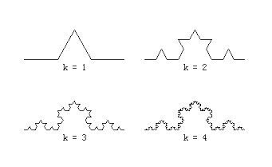
\includegraphics[width=0.7\linewidth]{pic/151409kzeswb2kzreg87zm.png}
	\caption{分形曲线}
	\label{fig:151409kzeswb2kzreg87zm}
\end{figure}


可以把这个k序列看作测量尺度变小的过程,计算不同k时计算的曲线长度$ L(K)=(4/3)^{K} $,所以Koch曲线的长度是无穷大。

\songti\setlength{\leftskip}{0em}

对于欧几里德空间$ \mathbb{R}^n $中的几何体,集合A的\textbf{Hausdorff测度}$ H^s(A) $定义如下:
\begin{equation}
	H_d^s(A)=\inf \left\{\sum_{i=1}^\infty |O_i|^s \mid \bigcup_{i=1}^\infty O_i \supset A, \;\; |O_i| \le d\right \},\; 
	H^s(A)=\lim_{d\rightarrow 0}H_d^s(A)
\end{equation}

$H^s(A) $定义在$ \mathbb{R}^n $的Borel集上,不难验证它满足可数可加性,所以是个带参数s的测度。当s=n时,$ H^s(A) $是$ \mathbb{R}^n $的n维勒贝格测度(精确地说只差一个与n有关的倍因子,因为Hausdorff测量的尺子是球,勒贝格是方块)。

在$ \mathbb{R}^n $空间,将几何体A线性放大k倍,其集合记为$ kA =\{kx \; | \; x\in A\} $,则有 $ H^s(kA)=k^sH^s(A) $,这与k维几何体的线性放大后,长度、面积和体积比例关系是一致的。注意到对于给定的集合A,Hausdorff测度$ H^s(A) $,随着s从n+1开始减小,其数值从0,到了一个临界点后,突然跳到无穷大,我们把这个s的临界值,称为几何体的维数,或者\textbf{Hausdorff维数}。当它是自然数时,这与我们日常中的经验是一致的,但有时它不是一个整数。

作为一个应用的例子,现在我们审视$ \mathbb{R}^n $空间里曲线的长度,凡是能够用积分算出有限值长度的,无论在平面或在三维空间,用Hausdorff测度可以证明都是一维的曲线。Koch曲线按照s=1来计算是无穷大,所以它可能是更高的维数。分形物体具有自相似结构,注意到如果将Koch曲线线性放大3倍,可以得到4份的原来曲线,根据上述s维几何体的线性放大与Hausdorff测度的倍数关系,可以算出$ s=ln4/ln3=1.26186... $,即Koch曲线是1.26186...维。前面例子中的康托集,线性放大3倍可以得到2份原来的康托集,所以它的维数是$ s=ln2/ln3=0.63093... $,是分数维的。只有在几何体所在的维度里的测度,才可能是一个正实数值。

如果你好奇,$ \mathbb{R}^n $空间里一个点的维数是多少?建议你用Hausdorff测度公式验算一下,以加深理解。只有s=0时,单点的Hausdorff测度是1,k个点和可数无穷个点,测度是k和无穷大,而它们在s>0时都是零测集。不可数的点集,在s=1时的测度,既可能为0,如康托集;也可能是正数,如有界区间;也可能是无穷大,如整条直线;还可能没有定义,如不可测集。这也许能给予古老的点与线段长度关系问题,更多一点的认识。

【扩展阅读】
\begin{enumerate}
	\item 维基百科,测度
	\url{http://zh.wikipedia.org/wiki/\%E6\%B5\%8B\%E5\%BA\%A6}
	
	\item  Wikipedia,Banach–Tarskiparadox \url{http://en.wikipedia.org/wiki/Banach\%E2\%80\%93Tarski_paradox}
	
	Wikipedia,Hausdorffmeasure 
	\url{http://en.wikipedia.org/wiki/Hausdorff\_measure}
	
	\item 维基百科,维塔利集合
	\url{http://zh.wikipedia.org/wiki/\%E7\%BB\%B4\%E5\%A1\%94\%E5\%88\%A9\%E9\%9B\%86\%E5\%90\%88}
	
\end{enumerate}

 	\chapter{重修微积分8——积分}

一元非负函数$ f(x) $从a到b的定积分,可以很直观地看成是这函数与x轴中[a,b]区间所夹的面积。在几何上,牛顿很直观地将[a,b]分割成细小的区间$ \Delta x $,以此为宽度的小长方块来填充或覆盖逼近这个面积,$ \sum_{i}f(x_i)\Delta x $,当Δx趋于零时它趋于这曲线所围的面积,莱布尼茨形象地把这个极限记为:$ \int_{a}^{b} f(x)dx $

。多元函数的多重积分是类推到高维体积的度量。

面积和高维体积按照这样计算的本质就是勒贝格测度。积分作为描述物理世界的数学模型,这是它所要求的属性。测度的计算是将整体切割成规范的部分,测算累加而成。上述牛顿的定义是按纵条切割的算法,叫做黎曼积分。面积也可以按横条来切割,把函数的值域区间细分,$ \sum _i  m(f^{-1}([y_i, y_i+\Delta y])) \Delta y $,算$ \Delta y $ 趋于零时的极限,这个算法收敛的极限叫勒贝格积分。(数学语言的定义见【1】,直观见图,图像来自网络下载)
\begin{figure}[h]
	\centering
	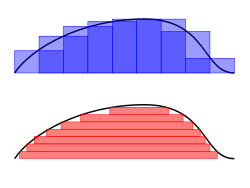
\includegraphics[width=0.7\linewidth]{pic/130332sliyik6hvp1iki1d.png}
	\caption{黎曼积分与勒贝格积分的直观区别}
	\label{fig:130332sliyik6hvp1iki1d}
\end{figure}

显然无论是用哪一种算法,它们计算所指的面积或体积是一样的,也应该相等的。将积分作为描述实践对象的数学模型,无论是用哪种测量计算方法,它们必须相等才有实用意义。这些面积或体积作为一种测度,如果按照不同的分割方法(即不同的积分定义)都有计算结果,在逻辑上也可证明是相等的。所以,如果黎曼积分和勒贝格积分都存在,它们相等。

如果函数具有负值,可以看成它是两个非负函数的相减。也就是两块面积体积或测度的相减,所以上述的结论也适用于一般的情况。

函数f在集合E上的勒贝格积分,记为$ \int_E f d m $,这里E是可测集,f是E上可测函数,m是E上的测度。当E是个区间时,它通常也用与黎曼积分相同形式的式子。请注意,对勒贝格积分,它只是沿用黎曼积分的形式记号,不再具有莱布尼茨那种对dx的符号解读。在可以缺省所指的测度和集合时,甚至将它记为$ \int_E f $或 $ \int f  $

因为所有黎曼可积的也是勒贝格可积,而且相等,借用相同积分形式的记法不会引起混淆。当你读论文里公式推导,看到不满足初等微积分相关的定理条件,居然也通行,不是作者不严谨,或误以为应用上不需要严谨,而是式子里指的是勒贝格积分。

勒贝格积分中测度、可测集,可测函数的术语吓住了许多对它们不熟悉的人,不敢使用。其实只要理解这是和黎曼积分一样应用,并具有更宽松应用条件的数学模型就不难了。黎曼积分的区域是可测集,能进行黎曼积分的函数是可测函数。黎曼积分都可写成勒贝格积分。在细节上:当E是一维时这里的勒贝格测度就是长度,二维时是面积,高维时是体积类推;说f是E上的可测函数,其定义是在E中f函数值大于任给一个数所有点形成的集合,都是可测集。大致说来,可测集包含了非数学专业人可以想象到的任何集合。迄今所知的勒贝格不可测集,都是用选择公理构造出来的无穷世界里的怪胎。如果你在物理或工程应用中涉及勒贝格积分,除非得到惊人违反常识的结果,大约都可放心地认为,你用到的都是可测集和可测函数。你大约还没有足够的运气和能力,构造出不可测集或不可测函数来犯错误。

既然这两种积分都一样,为什么黎曼积分用了几百年后,被称为经典分析而渐渐淡出,上个世纪初发展的勒贝格积分被广泛应用,并看作是近代分析的开端呢?

简单的答案是:应用黎曼积分在积分区域、积分函数及参与其他无穷过程时,有许多限制,而勒贝格积分解决了这些麻烦。它们是对相同应用的不同测算方法,就像原来用木尺丈量土地,现在改为用测距仪来测量一样,更有效的新方法必然会取代旧的,需要的只是熟悉。观念转换需要时间来消化,所读课本需要更新,个人则像是跟了不同师傅学了不同的功夫而已。

观念的不同带来了眼界的不同。经典分析一直徘徊在有限的视野和无穷的梦魇中。站在有穷世界的岸边,用无穷过程来窥视对岸的实无穷。想尽量保持有限世界的直观和逻辑上的严谨。这种囿于有限世界的观念和对无穷实质的回避,使得触及无穷时缩手缩脚,理论结果支离破碎。而勒贝格积分则基于包括有限和实无穷集合的测度研究上,以逻辑为骨架来拟合修正过去经验形成的概念。只要善于纠正陈旧观念形成的误区,在新的直观下,便能欣赏更广阔世界中简洁一致的美。

测度是从0到无穷大的量度。在包含着正负无穷大的扩充实数里,它们间的四则运算除了规定0乘无穷大仍为0外,其他都与中学关于无穷大的知识一致,包括了无穷大减无穷大没有定义。在勒贝格积分中,函数和积分的值域都是定义在这扩充的实数上。不难想象和证明,对于非负可测函数,勒贝格积分都存在。可测函数可以分解成两个非负可测函数之差,所以只要它俩的积分不都是无穷大,可测函数的积分都存在,在应用上都有意义。注意勒贝格积分存在,包括了它的积分值可能是无穷大的情况,所以勒贝格积分通常都存在。而勒贝格可积函数指的是积分值是有界的,显然,勒贝格可积等价于它是绝对可积的。

黎曼积分是定义在有界区间上有界函数的积分,这时勒贝格积分也有界,所以黎曼可积,勒贝格也是可积的。勒贝格积分定义在任何可测集上,包括可以黎曼积分的区间,和无界的全空间。黎曼积分要推广到无界的区间,它通常被定义为有界区间上积分的对称上下限无穷的扩展,在想象上比较直观,但这是个有疵瑕的形式扩展。例如,对于在0点从-1到1的阶跃函数,广义黎曼积分值是0,勒贝格积分不存在,对于周期函数也是如此。有些书上作为黎曼可积,勒贝格不可积的例子。但阶跃函数的广义黎曼积分,不满足平移不变性,若坐标向左或右平移一点,它的黎曼积分值就不同了。对周期函数如果黎曼积分的上下界不是对称地无穷扩展,它们的极限积分值也不一样。这用于描述物理世界,对应着测量的坐标变化和计算的方法不同,则意味着测算物理量的不同。所以对应于数学模型描述的对象,勒贝格不可积的结论正确地反映了这种不可计量的情况,广义黎曼积分则给出误导的答案。在推广到无穷的区域,广义的黎曼积分无论如何定义都有疵瑕。

黎曼积分最大的问题是,在与取极限、无穷级数、多重积分等运算的交换顺序,必须在很严格的条件下方为可行,这在应用上极不方便。实际上黎曼绝对可积的函数,在绝对值积分的范数下不是个完备的空间,这就像我们只在有理数域谈几何公式和代数应用,处处受到局限。从另一种观点来看,勒贝格积分可以定义为可积空间完备化的手段,它将函数绝对值黎曼积分为范数的计算方法更进,勒贝格可积函数是包含了黎曼可积函数的巴拿赫空间$ L^{1} $。【4】

为什么勒贝格积分会带来了这么多的便利?我们先用零测集牛刀小试。

黎曼积分在基本定义中假定被积的函数是连续的有界的,但应用中不一定都那么理想,可能有些间断点的“毛刺”,它的技术处理是分段来积分,然后将它们加起来,绕过这些疵点。在疵点是有限数目时,这样处理没有问题,但如果有无穷多个呢?

勒贝格积分告诉我们,如果这些疵点是零测集,把它们刨去换成任何数值,都不影响积分结果。黎曼积分和勒贝格积分如果同时存在,它们的数值必然相等。例如,Dirichlet函数D(x),当x是有理数时为1,无理数时为0;它在[0,1]区间的勒贝格积分为0,但不是黎曼可积的。我们知道可数个点集是零测集,有理数是可数的,所以是零测集,将这些点的函数值都置换成0,便是恒为0的常数值函数,这时黎曼积分也是0. 用这个方法“修理”黎曼积分中有疵瑕的函数,便得出黎曼积分的一个重要定理:

\kaishu\setlength{\leftskip}{1em}

区间[a,b]上函数f是黎曼可积的,必须且只需f在[a,b]上的不连续点是零测集。

\songti\setlength{\leftskip}{0em}


在积分和概率计算中都可以忽略零测集,这引入了常见的一个数学术语“几乎处处”(almost everywhere),简记为“a.e.”。如果两个函数不相等点的集合是零测集,叫做它们是“几乎处处相等”,它们的勒贝格积分相等。因此可以用一个几乎处处相等“良好的”函数来替代它计算。一个函数除了有个零测集外是有界的,叫做“几乎处处有界”。对积分的所有定理,可以把有界函数的条件换成“几乎处处有界”。闭区间上黎曼可积的函数,当且仅当是几乎处处连续的。

黎曼积分积分号里函数序列取极限,要在很强的条件下才能与积分号交换顺序。而“勒贝格控制收敛定理”说:在积分的集合上,只要它们的绝对值几乎处处不大于一个勒贝格可积函数,它们就几乎处处逐点收敛到一个函数,函数序列取极限就可以与勒贝格积分号交换顺序。

对于几乎处处一致有界的可测函数序列,勒贝格有界收敛定理给出更宽松的收敛要求,它只要这序列是按测度收敛就可以与积分号交换顺序了。什么是“按测度收敛”呢?就是说,这序列函数与其极限函数不同之处,将会趋于零测集。

对于$ \mathbb{R}^n $区间上勒贝格可积的函数,Fubini定理说,它的积分等于任何顺序的多重积分,也就是说可以任意地交换积分顺序。

牛顿—莱布尼茨公式描述了微分与积分的关系。记$ F'(x)=f(x) $,有 $ \int_a^b f(x)dx = F(b)-F(a) $ ,直观图像是,F曲线划分成n段折线,计算折线y轴上的增量与x轴增量之比,其导函数是当n趋近无穷大时,这些比值的极限。对这个导函数的积分,可以看成逼近导函数的这些折线比值与x轴增量的乘积累加的极限,很明显它是这些折线在y轴增量之和,因此等于这曲线在y轴数值之差。

在黎曼积分里这个定理要求被积函数在[a,b]上是连续的,或说原函数是连续可微的。在勒贝格积分里,我们有:原函数F在[a,b]上是绝对连续的,等价于它是勒贝格可积函数f的不定积分,且有牛顿—莱布尼茨公式关系。F几乎处处可导,其导数几乎处处等于f。这结论要比黎曼积分强多了,也更靠近直观想象。

仔细读过这篇文章,必要时将你应用积分推导的公式后面加个“(L)”,表明这是勒贝格积分,那么它“几乎处处”会让你免除许多严格条件限制的烦恼,和数学上不严谨的责难。

勒贝格积分除了与黎曼积分同样应用在$ \mathbb{R}^n $上,且有更自由积分区域外,还通用于任何定义有测度的抽象集合,例如随机过程在概率空间上的积分。勒贝格积分极大地提高了你的数学武功,只是你想深入其中纵横自如,则要走出历史旧观念的局限,改练无穷世界的测度基本功。


【扩展阅读】

\begin{enumerate}
	\item 维基百科,勒貝格積分
	\url{http://zh.wikipedia.org/wiki/\%E5\%8B\%92\%E8\%B2\%9D\%E6\%A0\%BC\%E7\%A9\%8D\%E5\%88\%86}
	
	\item 维基百科,维塔利集合\url{http://zh.wikipedia.org/wiki/\%E7\%BB\%B4\%E5\%A1\%94\%E5\%88\%A9\%E9\%9B\%86\%E5\%90\%88}
	
	\item 维基百科,微积分基本定理\url{http://zh.wikipedia.org/wiki/\%E5\%BE\%AE\%E7\%A7\%AF\%E5\%88\%86\%E5\%9F\%BA\%E6\%9C\%AC\%E5\%AE\%9A\%E7\%90\%86}
	
	\item 关肇直等,张恭庆,冯德兴,线性泛函分析入门,上海科学技术出版社,1979
\end{enumerate}


 	\chapter{重修微积分9---泛函}

算术是从一个或几个具体的数计算另一个数的学问,在这儿,数是已知和不变的。代数等式中有些数虽然未知,但其所指,仍是一个固定的数。在几百年前,只在几何中表示数量的对应,运动则代表着变化。几千年中的算术、几何和运动的研究,人们在三者间交叉借用形象来类比推理,直到1694年莱布尼茨终于用了函数这名词,抽象地表达变动的已知数到答案数之间,算法所对应的映射。其后近百年间,由约翰·伯努里和他的学生欧拉的推崇,最后到维尔斯特拉斯,确认了必须用函数的概念,把微积分建立在代数而不是几何的基础上。

函数,是我们从小学算术到中学要理解的第一个抽象概念,没过这坎的人,与数理绝缘,后面的课就不能理解了,对数学的认知停留在中世纪。初等微积分是在函数概念的基础上,对变动数极限运算的数学,牛顿称之为``流数术'',在有穷的世界窥测无穷的彼岸。近代分析建立在无穷空间的映射概念上,研究抽象空间结构和算子性质。由此俯视分析理论,能更抽象地构造数学模型,解决微分方程解和函数推广等等难题。理科生在这里,必须再过一个坎,走进抽象无穷的世界,才能理解现在的数学,而不是停留在二百年前的旧时光里。

算术的眼界局限在数域中。函数表达了数域中变量与映射值的对应关系。经典微积分用函数和极限的概念从数域,跨进实数和欧几里德空间。其运算都基于这个空间的性质。泛函分析将函数作为变量,研究它所在的空间和算子。在这里,一个函数也只看成集合上的一个点。

将讨论的对象抽象成集合中的点,点与点之间的相邻关系和点间运算对应关系,是集合上设定了的性质。数学的空间是定义有这些性质的集合,在这些设定条件下来讨论数学问题,而不再借助任何其他背景。在我们介绍过的空间里,由粗到精的包含关系顺序是:拓扑空间,$ T^2 $空间,距离空间,赋范空间,巴拿赫空间,希尔伯特空间。这些空间都只是抽象的类,可在相应的各类里设定具体的拓扑、距离、范数或内积。$ L^2 $和$ l^2 $空间,欧几里德空间,实数空间则是常见具体化的希尔伯特空间。初等微积分局限在实数空间和欧几里德空间里,泛函分析研究抽象的空间,特别是赋范空间、巴拿赫空间和希尔伯特空间的结构和线性运算性质。下面带你领略这里的风光。

两个距离空间中的映射称为算子。这篇只讨论赋范空间的线性算子。回顾一下赋范空间定义,它是线性空间,是以向量长度为范数导出了距离的距离空间。在这距离定义下,如果它对收敛还是完备的,则称为巴拿赫空间(Banach space)。大家熟悉的欧几里德空间$\mathbb{R}^n$,是有穷维的巴拿赫空间,其线性算子在基底下表示为矩阵。无穷维巴拿赫空间中线性算子的研究,是泛函分析的中心内容。

在分析中,函数是数与数的对应关系,是实数或复数间的映射,泛函则是以函数为自变量,对应于实数或复数值的映射。一般地说,从距离空间到数域的映射称为泛函。数域也是赋范空间,所以线性泛函也是一种线性算子。

\kaishu\setlength{\leftskip}{1em}

例9.1:函数的定积分是个线性泛函。下面$ L(f) $和$ K(f) $都定义了$ L^1[0,1] $空间上的一个泛函。(在[0,1]上绝对可积函数的空间上)

\songti\setlength{\leftskip}{0em}
\begin{equation}
	L(f)= \int_0^1f(t)dt \;\;\; \forall f \in L^1[0,1] \;\;\;\;\;\;
	K(f)= \int_0^1f(t)e^{-t}dt \;\;\; \forall f \in L^1[0,1]
\end{equation}

先介绍线性泛函的一些性质,以此来揭示赋范空间、巴拿赫空间和希尔伯特空间的结构。

对线性算子T,如果存在着一个正数c,对其定义域上所有的点都有$ \|Tx\| \leq c\|x\| $,称这个算子是有界的,这个c的下确界称为\textbf{线性算子T的范数}。对于线性算子,连续性与有界性是等价的。有界的算子总是把微小的变化映射成微小的差异,把有界的集合映射成有界的像。

泛函的连续性在应用上很重要,例如用一个收敛的函数序列来计算泛函作用下极限值,只有对连续泛函这样的逼近才有意义。欧几里德空间的线性泛函,可以表示成一个内积,它总是连续和有界的。但在赋范空间,并非所有的线性泛函都是有界或连续的。

\kaishu\setlength{\leftskip}{1em}

例9.2:闭区间[0,1]上连续可微函数集合$ C^1[0,1] $,以$ \|x\| = \max_{0\leq t \leq 1} \|x(t)\| $ 为范数构成赋范空间。函数在0点的导数是这空间的一个线性泛函。它不是连续的。因为对函数序列$ x_n(t)=\frac{1}{n}\sin(nt),n\geq 1 $,有$ \|x_n\| = \frac{1}{n} \rightarrow 0, \; n \rightarrow \infty $,即$ x_n \rightarrow 0 $,但是$ {x_n}'=\cos(n0)=1, \; n \geq 1 $ ,它并不趋于0。所以它不是连续的,也不是有界的。

\songti\setlength{\leftskip}{0em}

在某些线性距离空间,甚至没有非零的有界线性泛函。但是对赋范空间,我们却有足够多的有界线性泛函。

\textbf{Hahn-Banach延拓定理}:如果赋范空间的线性子空间上,定义有一个有界线性泛函,那么可以把它延拓到全空间,延拓后的算子也是个有界线性泛函,在原来子空间的映射保持不变,而且它的范数与延拓前是一样的。

取X中任何一个非零点$ x_0 $,它的数乘张成一维的线性子空间,在这子空间上定义一个有界线性泛函,使得$ f(x_0)= \|x_0\| $ ,应用这个定理,可以将它延拓到全空间,并且有$ \|f\| =1 $,这说明对于任何一个赋范空间,都有不比它向量少的有界线性泛函。

记赋范空间X上所有的有界线性泛函的集合为$ X^* $,不难验证$ X^* $在算子的范数下是一个巴拿赫空间。$ X^* $叫做X的\textbf{对偶空间},也称为\textbf{共轭空间}。$ X^* $的对偶空间$ X^{**} $,自然也是个巴拿赫空间。那么$ X^{**} $与X是什么关系?

对于X上的点x,可以定义$ X^* $上的泛函:$ L_x(f) = \overline{f(x)},\;\;  \forall f \in X^* $ 

显然,$ Lx $是线性的,而且$ \|Lx\| = \|x\| $,是有界的。这说明X到$ X^{**} $间有个一一的,线性的,并且保持范数相等的映射,即X等价于$ X^{**} $的一个线性子空间。如果这个映射还是满的,即X等价于$ X^{**} $,则称为X是\textbf{自反的},记为X=$ X^{**} $,自反的赋范空间必定是个巴拿赫空间。


\kaishu\setlength{\leftskip}{1em}

例9.3:函数空间$ L^p[0,1], p>1 $是自反的,它上面的线性泛函$ f(\cdot) $ 表示为
\[f(x)=\int_0^1 x(t)\overline{y(t)}dt, \;\;\; x\in L^p[0,1],\; y \in L^q[0,1], \;\frac{1}{p}+\frac{1}{q}=1\]

它的对偶空间是$ L^q[0,1] \;\; \frac{1}{p}+\frac{1}{q}=1 $

\songti\setlength{\leftskip}{0em}


自反巴拿赫空间与对偶空间互为有界线性泛函的关系,让我们联想起内积的关系。所以就用内积的符号来表示线性泛函,$f(x)=\langle x,f\rangle$
,对它们间的线性性质与内积形式上完全一样,只不过这里左右矢量是在不同的空间。特别地,从线性算子范数的定义,有与内积完全相同的Schwarz不等式$  |\langle x,y\rangle |\leq \|x\|\|y\| $

希尔伯特空间H是定义了内积,并以此导出范数的巴拿赫空间。由上面巴拿赫空间与对偶空间的内积表示,及Schwarz不等式,很自然地会猜测:H空间的对偶空间是否是它自己?确实如此。H中任何一点,都可以用内积定义H空间上的一个有界线性泛函,这说明H是H*的子集。\textbf{Riesz表现定理}则证明,H空间上,任何一个有界线性泛函$ f\in H^* $,都对应着空间中的一个点$ y\in H $,使得$ f(x)= \langle x,f\rangle ,\forall x\in H $,而且$ \|f\| = \|y\| $,这说明$ H^* $是$ H $的子集。所以$ H=H^* $。

Hahn-Banach延拓定理证明了每一个巴拿赫空间,它的有界线性泛函构成了它的对偶的巴拿赫空间,有界线性泛函算子间的作用可以用内积的式子来表示。Riesz表现定理则肯定了希尔伯特空间的对偶空间就是它自己。Hahn-Banach延拓定理可以放宽到,具有线性的距离空间附加上一些条件,泛函分析的教科书介绍这方面的内容。

距离空间中收敛的要求比较强,用泛函我们可以定义一种比较弱的``功能性''的收敛。

比如说,赋范空间X中的序列$ (x_n) $收敛于$ x_0 $,指 $ \lim_{n\rightarrow \infty}\| x_n - x_0 \| $

这有时称为\textbf{强收敛},\textbf{弱收敛}则定义为这序列对所有的有界线性泛函都有

\[\lim_{n\rightarrow\infty}f(x_n) = f(x_0),\;\; \forall f \in X^*\]

$ X^* $中序列$ (f_n) $ \textbf{弱*收敛}于$ f_0 $,则是满足

\[\lim_{n\rightarrow\infty}f_n(x) = f_0(x),\;\; \forall x \in X\]

显然强收敛隐含着弱收敛,弱收敛未必能强收敛,下面是个例子。

\kaishu\setlength{\leftskip}{1em}

例9.4:希尔伯特H的任何正交归一基{ $ e_n $ },不难从向量在这个基上分解的无穷序列和中得到,$ \lim_{n\rightarrow\infty}\langle x,e_n \rangle =0,\;\forall x\in H $

由Riesz表现定理得知,这表明这基的序列弱收敛于0,但是所有基向量的范数都是1,所以它不可能强收敛于0.

\songti\setlength{\leftskip}{0em}


【扩展阅读】

\begin{enumerate}
	\item 关肇直等,张恭庆,冯德兴,线性泛函分析入门,上海科学技术出版社,1979
	
	\item 程代展,系统与控制中的近代数学基础,北京:清华大学出版社,2007 \url{http://product.dangdang.com/9350967.html}
	

\end{enumerate}


	转载本文请联系原作者获取授权,同时请注明本文来自应行仁科学网博客。
链接地址:\url{http://blog.sciencenet.cn/blog-826653-892196.html }
 	\section{重修微积分10——算子}

算术是从给定条件和已知数,得出符合条件数值,计算的学问。算法用给定的条件,构造性地定义了从已知数到得数的映射。算术所在的数域仅仅是抽象空间包含的一个实例。近代分析把抽象空间作为给定条件,定义在空间的映射称为算子,研究它们的一般性质。

例如,迭代算法是用相同的子算法,把得数作为下次计算的已知数,一次次地迭代计算来逼近结果的计算方法。抽象空间里的压缩映像是能够应用于这类计算的算法。

距离空间 $ (X,d) $ 具有如下性质的映射称为\textbf{压缩映像} $ T: X \rightarrow X, \;$  $\; d(Tx, Ty)\leq ad(x,y) $,  $ a\in(0,1),\forall x,y \in X $。这里的$ d(x,y) $是x和y间的距离,如差值的绝对值及范数等等。应用压缩映像不断地迭代计算,能够逼近至多一个不动点。巴拿赫不动点原理说,压缩映像T在完备距离空间X中,有唯一的不动点$ x $,即 $  Tx = x $. 有了压缩映像T,在X中任取一点$ x_0 $,令$ x_{n+1} =Tx_n, n=0,1\cdots $,它将收敛于一个不动点$ x $.重要的原理都是简单和直观的。这个定理在分析中是个强有力的工具,以此可以证明空间和流形上的各种的反函数定理,它不仅可用来定性地证明常微分方程解的存在和唯一性,而且是解方程迭代算法的基础。

压缩映像是个算子,可以是线性也可以是非线性的。但在分析中,研究最多并最富有成果的是无穷维空间的线性算子。

为什么要研究无穷维空间的线性算子呢?因为物理的动态系统从初始状态开始的变化,微分方程由状态函数映射成微分关系和边界条件,工程系统由输入转变成输出,都可以看成一个算子作用在函数空间进行变换。出自叠加原理应用和近似的简化,这些算子也多是线性的。微分和积分作为算子是线性的,它们与其他因子组合而成的算子,例如傅立叶变换,拉普拉斯变化等积分变换,线性常微分方程,数理方程,这些数学工具都是无穷空间的线性算子。

数学上,代数关心的是集合中元素在运算映射下的性质。分析则研究这些代数运算在无穷空间中变动极限的性质。这就要考虑集合所在空间的拓扑性质,和了解在这些代数运算角度下空间的结构。上一篇,我们用有界线性泛函的内积形式,揭示了巴拿赫空间以及希尔伯特空间的对偶关系。这里要介绍线性算子的基本性质。

请注意,空间的线性,是集合中的元素对线性运算封闭,例如连续函数集合是线性空间,因为连续函数的数乘和相加仍然是连续函数。而算子的线性,则是算子的映射对空间上的线性运算保持不变的关系,即线性组合的映像等于组合中元素映像的线性组合,例如积分是在闭区间连续函数空间上的线性算子,线性常微分方程的系数可以是非线性的函数。线性算子必须作用在线性空间上,而线性空间上的算子可以是非线性的。

复习一下这里要用到的几个空间的概念。距离空间在集合任意两点中定义有距离,以此定义开球和邻域,生成空间的拓扑。赋范空间是线性空间,是以向量长度为范数导出了距离的距离空间。在这距离定义下,如果它对收敛还是完备的,则称为巴拿赫空间(Banach space)。希尔伯特空间是定义有内积的巴拿赫空间。这篇谈定义在赋范空间上的线性算子。线性代数课程讨论问题在欧几里德空间,它是有穷维的巴拿赫空间$ \mathbb{R}^n $,其线性算子在基底下表示为矩阵,它只是局限在有穷维的表现,我们对比地来介绍一般的线性算子。

上篇说过,对线性算子T,如果存在着一个正数c,对其定义域上所有的点都有$ \|Tx\| \leq c\|x\| $,则这个算子是有界的。这个c的下确界称为\textbf{线性算子}T\textbf{的范数}。

欧几里德空间上的线性算子都是连续的和有界的,这在巴拿赫空间未必成立。

\kaishu\setlength{\leftskip}{1em}

例10.1:闭区间[0,1]上连续函数集合C[0,1],以$ \|x\|_\infty = \max_{0\leq t \leq 1} |x(t)| $ 为范数构成巴拿赫空间。定义在C[0,1]到C[0,1]的微分算子D,是这空间上的线性算子,它的定义域是在 C[0,1]中所有连续可微函数构成的线性子空间。D不是有界的。因为函数序列{$ x_n(t)|x_n(t)=e^{−nt}, n\geq 1 $}在C[0,1]中,有$ \|xn\|_\infty =1 $,不难推出它是个有界的集合(这集合中任何两点的距离都小于2),但是$ Dx_n(t)=\frac{d}{dt}x_n(t)=−nx_n(t) $ 的集合,却是C[0,1]中的无界集。算子D将有界的集合映射成无界的像,所以它是无界的算子。

\songti\setlength{\leftskip}{0em}

线性算子是否有界,还取决于映射所在空间的拓扑。微分算子D定义在另一范数的空间,可以是有界的。

\kaishu\setlength{\leftskip}{1em}

例10.2:连续函数集合$ C[0,1] $以范数$ \|x\|_\infty $,构成巴拿赫空间。记函数x的导数为x’,连续可微函数集合$ C^1[0,1] $的范数定义为$\|x\|1= \|x\|_\infty +\|x′\|_infty$ ,它也是个巴拿赫空间。

微分算子D也是$ C^1[0,1] $空间到$ C[0,1] $上的线性算子,有
\[\|Dx\|_\infty =\|x′\|_\infty \leq \|x\|_\infty +\|x′\|_\infty =\|x\|_1,\forall x \in C^1[0,1]\]
这说明$ C^1[0,1]$空间中有界的集合,在算子D映射下在$ C[0,1] $上仍然是有界的,所以它是这空间里有界的算子。

\songti\setlength{\leftskip}{0em}

尽管赋范空间中线性算子不一定是有界的,但有界性和连续性却是等价的,甚至只要在某一点上连续,它们就有了全体的连续性和有界性。

在欧几里德空间,线性算子$ T $,用下面的内积式子,可以定义它的对偶算子$ T^* $,
\begin{equation}
	\left\langle Tx, y \right \rangle = \left \langle x, T^* y \right \rangle, \;\;\;  \forall x \in \mathbb{R}^n, \;\; \forall y \in \mathbb{R}^m
\end{equation}

用矩阵表示,$ T^* $是$ T $的共轭转置矩阵。对于赋范空间,我们也对线性算子用相同的方法定义其对偶算子。不过从空间X到Y的算子不一定对全空间都有定义,例如在微分算子T在连续函数空间$ C[0,1] $,只对其中连续可微的函数有定义。上述的定义只限在各自的定义域里。

算子$ T $的定义域记为$ D(T) $。如果$ D(T) $是稠集,即空间X中任何一个点,都可以表示为$ D(T) $中点序列的极限,$ T $则称为是\textbf{稠定}的。赋范空间X到巴拿赫空间Y上的有界线性算子,如果是稠定的,它可以唯一地(按连续性)延拓到整个空间,成为定义在X上的有界算子,且算子的范数与原来的相等。

如果$ T $的值域充满了Y的全空间,则称为是满的。如果$ D(T) $中的序列$ (x_n) $当$ x_n \rightarrow x,Tx_n \rightarrow y $,有$ x $也在$ D(T) $中,$ Tx=y $,则称$ T $是闭的。\textbf{闭算子}定义域中所有的点$ x $与对应像$ Tx $的组合$ (x, Tx) $,在$ X\times Y $空间中是个闭集。

如果$ T $是两个希尔伯特空间中的线性算子,T是稠定的则$ T^* $是闭的,如果$ T $还是闭的,则$ T^* $也是稠定的,而且有$ T^{**}=T $。

欧几里德空间上的线性算子,可以表达成矩阵A,其范数$ \|A\| $
是它与共轭转置矩阵相乘$ A’A $最大特征值的开平方值,它们的全体也是个欧几里德空间。相应的,赋范空间X到巴拿赫空间Y上的有界线性算子,所有这些有界线性算子$ L(X,Y) $,在算子的范数下也是巴拿赫空间。

微分方程可以看成算子T作用在线性距离空间的点上,等于另一空间的点(函数,初始或边界条件),例如Tu = v。应用算子理论研究微分方程,解的存在性对应着算子T有右逆,解的唯一性对应着算子T有左逆,所以T的逆算子存在意味着解的存在和唯一性。解的稳定性说,当参数、边界或初始条件变化很小时,解也应该变化很小,这对应着逆算子的连续性即有界性。在未知是否有逆时,稳定性的要求表达成算子的开映像性质,而微分方程解对初值一致连续性则表达成算子族的一致有界性。

这些问题,对于巴拿赫空间X到Y的线性算子T,都已经有了很好的答案。

\textbf{开映像定理}:如果T是闭的和满的,对于任意小的 $ \epsilon >0 $,有相应的 $ \delta >0 $,使得
\begin{equation}
	\forall y\in Y, \; \left \| y \right \| < \delta \Rightarrow \exists x \in D(T), \; \left\|x\right\|<\epsilon , \; y=Tx
\end{equation}

简言之,开集的像是开的。

\textbf{巴拿赫逆算子定理}:如果T是闭的,满的,一一对应的,则它的逆算子存在且是有界的。

\textbf{闭图像定理}:如果T是闭的,定义域是X全空间,则T是有界的。

\textbf{共鸣定理}:如果一族有界线性算子在X上是逐点有界的,那它们也是一致有界的。

上述这几个是泛函分析中线性算子的基本定理。它们都还有在更广泛的线性距离空间,附加上一些条件的版本。有兴趣请看泛函分析的教科书。

线性算子的这些性质,让线性微分方程成为描述世界强有力的工具。在这种线性描述下,逆算子的存在,证明了一切的变化都可以由已知的原理、参数、边界和初始条件唯一地确定;逆算子的连续性保证了一切的误差都是可以无限地消减。这个关于无穷过程线性数学利器的成功应用,让人们相信世界是确定性的,无穷可分的,差不多是线性的,几乎忘记了为了能够应用这个利器,曾经省却了一些细节,作过了一些假设,即使非线性的研究也只往这方向靠,忽略本质不同难以想象的部分,直至非线性动力系统以混沌、分叉、孤立子突兀在眼前,打破了幻想,在数学上揭示了系统上不确定的机制。

三百多年前,微积分以函数为阶梯从无穷小分析的思路,把人们带进了想象中的无穷世界。由线性联系着微观机制和宏观的表现,线性系统的叠加原理所惠,让它成为研究动态和连续系统最强有力的工具。短短的三百年时间,研究函数科学的分析,成为数学最大的分支。在这无穷可分几乎是线性的世界里,数学分析是撰写自然律法的笔墨文书,是从事理工研究必不可少的工具。我们对世界的认知,其实是符号的象征和想象的产物,数学工具极大地影响着研究者对事物构造的想象和规律的理解,进而推及大众。计算机的出现,将可能改变世界的图像,影响着数学研究方向和对世界的认知。世界也许将回到有穷分立的结构,非线性将是主流,复杂和不确定系统或成为富饶的主题。但无论怎么改变,数学都是人们用逻辑来及远的工具,指使计算机的方向,描绘世界的画笔。现在的计算机在科研中,还基本是分析计算的工具,图像表达的机器和记忆搜索的助手。人们还未找到代替叠加原理超越线性,组合分立研究结果的方法,还在等待着一个革命性的思想,来指引怎样用计算机来描述,理解和控制我们的世界。在这之前,数学分析仍然统治着物理和工程的世界,理科生还离不开这时代战士必备的这个武器。



【扩展阅读】

\begin{enumerate}
	\item 关肇直等,张恭庆,冯德兴,线性泛函分析入门,上海科学技术出版社,1979

	\item 程代展,系统与控制中的近代数学基础,北京:清华大学出版社,2007 
	\url{http://product.dangdang.com/9350967.html}


\end{enumerate}

转载本文请联系原作者获取授权,同时请注明本文来自应行仁科学网博客。
链接地址:http://blog.sciencenet.cn/blog-826653-893883.html 
\end{document}